% chapter3.tex -- de (German)
\chapter{Installation der Software}
Eigentlich ist die Installation der Software \textit{babyleicht} und man
muss (Achtung: Unwort!) \textit{nur} den \cmd{one-line-installer} von
\textit{MiczFlor} auf einem jungfr�ulichen \os{Raspbian} starten\dots\\
\url{https://github.com/MiczFlor/RPi-Jukebox-RFID#installation}

\textbf{Aber:}\\
Aufgrund vieler Anfragen der mittlerweile relativ gro�en Community rund
um die {\Bezeichnung} und der daraus resultierenden zahlreichen
\textit{Push Requests} auf github und auch wegen vieler anderer guter
Gr�nde schleichen sich in die an sich gro�artige Arbeit von
\textit{MiczFlor} naturbedingt immer wieder kleinere Fehler ein, die
insbesondere f�r unbedarfte Neulinge bisweilen schwer zu finden und zu
beseitigen sind.

%\begin{bclogo}[logo = \bclampe, noborder = true]{Hinweis}
F�r die Installation der Software m�ssen einige Konfigurationsdateien
angepasst werden. Im git-Repository unter
\url{https://github.com/schlizbaeda/schlizbaedas_Phoniebox} gibt es das
Unterverzeichnis \filenam{files}, in dem diese Dateien in dem Stand
enthalten sind, wie sie auf {\autor}s {\Bezeichnung} produktiv
eingesetzt werden. %Anstatt die Konfigurationsdateien selbst zu
%editieren, wie im diesem Kapitel beschrieben, k�nnen auch diese Vorlagen
%verwendet werden.
%\end{bclogo}
\begin{table}[h]
\centering
\renewcommand{\arraystretch}{1.11}
\begin{tabular}{|p{0.55\textwidth}|p{0.35\textwidth}|p{0.1\textwidth}|}
\hline
\textbf{/absoluter Pfad/Dateiname}	&	\textbf{Verwendung}								&	\textbf{wo?}\\
\hline
\filenam{/boot/wpa-supplicant.conf}	&	t.b.d.	&	\\
\hline
\filenam{/boot/config.txt}			&	allgemeine Konfigurationsdatei\newline des \RPi	&	link\\
\hline
\filenam{/etc/asound.conf}			&	t.b.d.	&	\\
\hline
\filenam{/home/pi/RPi-Jukebox-RFID/requirements.txt}	&	t.b.d.	&	\\
\hline
\filenam{/etc/lighttpd/lighttpd.conf}	&	Web-App der \Bezeichnung	&	\\
\hline
\filenam{/etc/sudoers}					&	t.b.d.	&	\\
\hline
\filenam{/etc/lighttpd/conf-available/15-fastcgi-php.conf}	&	t.b.d.	&	\\
\hline
\filenam{/etc/mpd.conf}				&	t.b.d.	&	\\
\hline
\filenam{/home/pi/RPi-Jukebox-RFID/scripts/gpio-buttons.py}	&	t.b.d.	&	\\
\hline
\filenam{rfid\_trigger\_play.conf}	&	In dieser Datei ist die Syntax erkl�rt	&	\\
\hline
\filenam{/etc/rc.local}					&	Autostart: Starten von \filenam{onoffshim\_switch.sh}	&	\\
\hline
\filenam{/home/pi/onoffshim\_switch.sh}	&	{\onoffshim} cyberghost	Teil 1	&	\\
\hline
\filenam{.../onoffshim\_gpio-shutoff.sh}		&	{\onoffshim} cyberghost	Teil 2	&	\\
\hline
\end{tabular}
\vspace{0.5cm}
\caption{Konfigurationsdateien von {\autor}s \Bezeichnung}
\label{tab:cfgfiles}
\end{table}
\todo{Tabelle vervollst�ndigen}TODO:

% chapter3_01.tex -- de (German)
% installation of Raspbian Buster Lite
\section{\os{Raspbian Buster Lite} auf dem {\RPi} installieren}
Einige Tutorials im Internet empfehlen zwar, die Software f�r die
{\Bezeichnung} unter \os{Raspbian Buster with desktop} zu installieren,
aber da es sich bei der {\Bezeichnung} um ein einfaches
stand\-alone-System ohne Bildschirm handelt, ist es in meinen Augen
v�llig ausreichend, die Installation auf dem wesentlich kleineren
\os{Raspbian Lite} vorzunehmen. Ein grafischer X11-Desktop ist
schlichtweg nicht erforderlich. Au�erdem reicht f�r \os{Raspbian Buster
Lite} zur Not sogar eine SD-Karte mit einer Speicherkapazit�t von 4GB.

\subsection{Erstellen einer SD-Karte mit \os{Raspbian Buster Lite}}
Zun�chst wird die aktuelle Version von \os{Raspbian Buster Lite} von der
Homepage der {\foundation}
(\url{https://www.raspberrypi.org/downloads/raspbian/}, ca. 450MiB)
heruntergeladen und entpackt (1,8GiB). Das entpackte Image wird mit
einem daf�r vorgesehenen Programm wie \software{win32diskimager} oder
am Linux-PC mit dem systemeigenen Kommando \cmd{dd} auf die SD-Karte
\textit{geflasht}, um das Image 1:1 zu �bertragen.
\begin{bclogo}[arrondi = 0.2, logo = \bcinfo, ombre = true, epOmbre = 0.25, couleurOmbre = black!30,blur]{Achtung}
Es reicht nicht, die Imagedatei einfach auf eine bereits formatierte
SD-Karte zu kopieren!
\end{bclogo}
Die Details des \textit{Flashens} von Betriebssystem-Images auf eine
SD-Karte werden von der {\foundation} unter
\url{https://www.raspberrypi.org/documentation/installation/installing-images/README.md}
ausf�hrlich beschrieben und in diesem Dokument als bekannt
vorausgesetzt.

Nach dem Flashen enth�lt die SD-Karte zwei Partitionen:
\begin{compactitem}
\item{die FAT32-formatierte \filenam{/boot}-Partition}
\item{die ext4-formatierte Rootpartition von \os{Raspbian}}
\end{compactitem}
\begin{bclogo}[logo = \bclampe, noborder = true]{Hinweis}
Beim (erneuten) Anstecken der SD-Karte am PC werden diese beiden
Partitionen im Dateimanager angezeigt. Sollte auf dem PC jedoch das
Betriebssystem \os{Windows} verwendet werden, so wird nur die
FAT32-formatierte \filenam{/boot}-Partition erkannt.
\end{bclogo}


\newpage
\subsection{Anmeldung am {\RPi} �ber \software{ssh}}
\begin{bclogo}[logo = \bclampe, noborder = true]{Hinweis}
F�r die ersten Schritte muss die Netzwerkverbindung zum {\RPi} �ber ein
verkabeltes LAN aufgebaut werden, da die WLAN-Verbindung noch nicht
eingerichtet ist! Dies geschieht erst in Abschnitt \ref{sect:setupWLAN}.
\end{bclogo}
\begin{figure}[h]
\centering
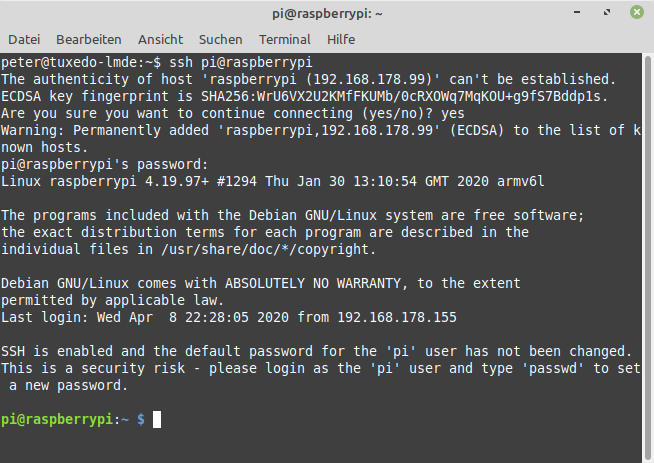
\includegraphics[width=0.90\textwidth, angle=0]{software/login.png}
\caption{erster Login �ber \software{ssh}}
\label{fig:ssh_login}
\end{figure}
Da an den {\RPi} f�r die {\Bezeichnung} weder Bildschirm noch Tastatur
angeschlossen werden, muss der Zugriff auf den {\RPi} von Anfang an �ber
\software{ssh} erfolgen. Dazu muss auf der Partition \filenam{/boot} der
SD-Karte die leere Datei \filenam{ssh} angelegt werden.\\
Nun wird die SD-Karte in den {\RPi} gesteckt, der {\RPi} \textbf{�ber
Ethernet ans LAN} geh�ngt und eingeschaltet. Nach sp�testens einer Minute
sollte \os{Raspbian Buster Lite} vollst�ndig gebootet und der {\RPi} im
LAN bekannt sein. Auf dem PC wird in einem Terminalfenster
(unter \os{Windows} in der Eingabeaufforderung \cmd{cmd.exe}) die
Software \software{ssh} mit folgendem Kommando gestartet:

\cmdPC{ssh pi@raspberrypi}\comment{Das Passwort lautet \texttt{raspberry}}

Die Bildschirmausgabe sieht in etwa wie in Abbildung \ref{fig:ssh_login}
aus.


\newpage
\subsection{\os{Raspbian} konfigurieren}
Nach erfolgreichem \software{ssh}-Login muss das System jetzt auf einen
aktuellen und sicheren Stand gebracht werden:\\
\cmdPi{sudo apt update \&\& sudo apt upgrade}\comment{System auf den neuesten Stand bringen}\\
\cmdPi{sudo raspi-config}\\
\stdout{1 Change User Password \ \ \ \ \ \ \ \ \ \ \ \ \ \ \ \ \ \ \ \ \ \ \ \ \ \ \ }\comment{Passwort unbedingt �ndern!}\\
\stdout{2 Network Options \ \ \ \ \ --> N1 Hostname \ \ \ \ \ \ \ \ \ \ \ \ }\comment{\zB \texttt{phoniebox1}}\\
\stdout{3 Boot Options \ \ \ \ \ \ \ \ --> B1 Desktop / CLI \ \ \ \ \ \ \ \ --> B2 Console Autologin}\\
%\stdout{4 Localisation Options --> I1 Change Locale \ \ \ \ \ \ \ }\comment{Landeseinstellungen}\\
\stdout{4 Localisation Options --> I2 Change Timezone \ \ \ \ \ }\comment{Zeitzone anpassen}\\
\stdout{\textcolor{white}{ \ \ \ \ \ \ \ \ \ \ \ \ \ \ \ \ \ \ \ \ \ \ } --> I4 Change Wi-fi Country }\comment{diese Anpassung ist ganz wichtig!}\\
\stdout{5 Interfacing Options \ --> P2 SSH}

Beim Verlassen von \software{raspi-config} sollte die Abfrage 
\texttt{Would you like to reboot now?} mit \button{yes} beantwortet
werden. Der {\RPi} wird neu hochgefahren. Vom PC aus kann nach ca.
einer Minute Wartezeit ein neuer \software{ssh}-Login auf den neuen
Hostnamen mit dem (hoffentlich) ge�nderten Passwort erfolgen:\\
\cmdPC{ssh pi@phoniebox1}

\subsection{WLAN einrichten}
\label{sect:setupWLAN}
Da die {\Bezeichnung} als tragbares Ger�t f�r's Kinderzimmer konzipiert
ist, sollte ein WLAN-Zu\-gang eingerichtet werden, um als Eltern sp�ter
\zB per Laptop oder Smartphone jederzeit einen \textit{bequemen}
Zugriff auf die Box zu haben. Wie h�ufig unter \os{Linux} gibt es auch
f�r die WLAN-Konfiguration mehrere zielf�hrende Wege, wie sie \zB im
Elek\-tro\-nik-Kom\-pen\-dium unter
\url{https://www.elektronik-kompendium.de/sites/raspberry-pi/1912221.htm}
beschrieben werden. F�r {\autor}s {\Bezeichnung} wird die dort
beschriebene "`Variante 2"' mittels \software{wpa\_supplicant}
verwendet.

Auf einem frisch installierten \os{Raspbian Lite} wird der WLAN-Zugriff
in der \software{ssh}-Konsole  �ber die Datei
\filenam{ /etc/wpa\_supplicant/wpa\_supplicant.conf} eingerichtet. Die
drei ersten Zeilen sollten in der Datei bereits vorhanden sein. F�r
jedes gew�nschte WLAN muss ein Eintrag \texttt{network\{\dots\}} nach
folgendem Schema eingef�gt werden. Dazu wird der auch �ber
\software{ssh} funktionierende Texteditor \software{nano} verwendet:\\
\cmdPi{sudo nano /etc/wpa\_supplicant/wpa\_supplicant.conf}\\
\editor{ctrl\_interface=DIR=/var/run/wpa\_supplicant GROUP=netdev\\
        update\_config=1\\
        country=DE\\
        \\
        network=\{ \# Erweiterungen von \autor\\
        \textcolor{white}{\ \ \ \ }ssid="{<wlan-name>}" \ \# Klartext-Bezeichnung des Netzwerkes\\
        \textcolor{white}{\ \ \ \ }psk="{<passphrase>}" \ \# Passwort f�r WLAN-Zugriff\\
        \textcolor{white}{\ \ \ \ }key\_mgmt=WPA-PSK\\
        \}
       }
       
Um diese Einstellungen tats�chlich zu aktivieren, m�ssen im Anschluss
folgende Kommandos abgesetzt werden:\\
\cmdPi{sudo systemctl restart dhcpcd}\\
\stdout{\textcolor{red}{Warning:} The unit file, source configuration
        file or drop-ins of dhcpcd.service changed on disk. Run
        'systemctl daemon-reload' to reload units.}\\
\cmdPi{sudo systemctl daemon-reload}\comment{gem�� obiger Warnung}\\
\cmdPi{ip addr}\\
\stdout{1: lo: <LOOPBACK\,UP\,LOWER\_UP> mtu 65536 qdisc noqueue state UNKNOWN group default qlen 1000\\
        \textcolor{white}{\ \ \ \ }link/loopback 00:00:00:00:00:00 brd 00:00:00:00:00:00\\
        \textcolor{white}{\ \ \ \ }inet 127.0.0.1/8 scope host lo\\
        \textcolor{white}{\ \ \ \ \ \ \ }valid\_lft forever preferred\_lft forever\\
        \textcolor{white}{\ \ \ \ }inet6 ::1/128 scope host\\
        \textcolor{white}{\ \ \ \ \ \ \ }valid\_lft forever preferred\_lft forever\\
        2: eth0: BROADCAST\,MULTICAST\,UP\,LOWER\_UP> mtu 1500 qdisc pfifo\_fast state UP group default qlen 1000\\
        \textcolor{white}{\ \ \ \ }link/ether b8:27:eb:36:6f:a7 brd ff:ff:ff:ff:ff:ff\\
        \textcolor{white}{\ \ \ \ }inet 192.168.178.153/24 brd 192.168.178.255 scope global dynamic noprefixroute eth0\\
        \textcolor{white}{\ \ \ \ \ \ \ }valid\_lft 859570sec preferred\_lft 751570sec\\
        \textcolor{white}{\ \ \ \ }inet6 fe80::3a9f:9d8c:1f44:e940/64 scope link \\
        \textcolor{white}{\ \ \ \ \ \ \ }valid\_lft forever preferred\_lft forever\\
        3: wlan0: <BROADCAST\,MULTICAST\,UP\,LOWER\_UP> mtu 1500 qdisc pfifo\_fast state UP group default qlen 1000\\
        \textcolor{white}{\ \ \ \ }link/ether b8:27:eb:63:3a:f2 brd ff:ff:ff:ff:ff:ff\\
        \textcolor{white}{\ \ \ \ }inet 192.168.178.154/24 brd 192.168.178.255 scope global dynamic noprefixroute wlan0\\
        \textcolor{white}{\ \ \ \ \ \ \ }valid\_lft 863877sec preferred\_lft 755877sec\\
        \textcolor{white}{\ \ \ \ }inet6 fe80::b04c:315b:a4c9:3c9d/64 scope link\\
        \textcolor{white}{\ \ \ \ \ \ \ }valid\_lft forever preferred\_lft forever
       }

Damit ist die {\Bezeichnung} f�r den k�nftigen WLAN-Zu\-griff
freigeschaltet. Der bis jetzt verwendete LAN-Zu\-griff �ber das
Ethernetkabel ist ab sofort nicht mehr notwendig. Zum Test wird die
laufende \software{ssh}-Sitzung beendet, das Ethernetkabel abgesteckt
und eine neue \software{ssh}-Sitzung gestartet:\\
\cmdPi{exit}\comment{Schlie�en der bestehenden ssh-Sitzung �ber LAN}\\
\textit{Jetzt das Ethernetkabel abstecken!}\\
\cmdPC{ssh pi@phoniebox1}\comment{neue ssh-Sizung �ber WLAN �ffnen}

%\begin{bclogo}[arrondi = 0.2, logo = \bcinfo, ombre = true, epOmbre = 0.25, couleurOmbre = black!30,blur]{Achtung}
\begin{bclogo}[logo = \bclampe, noborder = true]{Hinweis}
Entgegen vieler Tutorials wurde bei {\autor}s {\Bezeichnung} auf die
Zuteilung einer statischen (festen) IP-Adresse verzichtet! Stattdessen
wird von der {\Bezeichnung} beim Bootvorgang �ber DHCP eine dynamische
IP-Adresse angefordert, um den Netzwerkzugriff m�glichst flexibel zu
halten. Die konkret vergebene IP-Adresse kann mit dem Kommando
\cmd{ip addr} ermittelt werden und lautet im obigen Beispiel
\texttt{192.168.178.154}.
\end{bclogo}

% chapter3_02.tex -- de (German)
% OnOffSHIM
\section{\onoffshim}
\label{sect:onoffshim_software}
Der {\onoffshim} ist ein kleines Erweiterungsmodul, das ein komfortables
Ein- und Ausschalten inklusive sauberem Herunterfahren des {\RPi} 
erm�glicht:\\
\url{https://shop.pimoroni.com/search?type=product&q=onoffshim}\\
Prinzipiell ist dieses Modul vom Konzept her gut durchdacht
und f�r batteriebetriebene \RPi-Projekte gut geeignet. Allerdings f�hrte
bei mir ein zu langes Bet�tigen des On-/Off-Tasters dazu, dass der
{\onoffshim} die Spannungsversorgung nicht vollst�ndig ausschaltete,
siehe Abschnitt \ref{sect:onoffshim_relay}.

\begin{bclogo}[arrondi = 0.2, logo = \bcinfo, ombre = true, epOmbre = 0.25, couleurOmbre = black!30,blur]{Achtung}
Die hier beschriebene Installation der Software verwendet \textbf{nicht}
die Originalsoftware des Herstellers \textit{Pimoroni}, sondern eine
Variante, die unter
\begin{smaller}\url{https://retropie.org.uk/forum/topic/15727/tutorial-onoff-shim-exposed-neat-powerswitch-from-pimoroni/}\end{smaller}\\
beschrieben wird!
\end{bclogo}

Vom Hersteller \textit{Pimoroni} wird zwar auch eine Software
mitgeliefert, die als Linux-Daemon (Hintergrunddienst) arbeitet und mit
folgendem Kommando aus dem Internet heruntergeladen und installiert
werden k�nnte:\\
\cmdPi{curl https://get.pimoroni.com/onoffshim | bash}
\comment{wurde so nicht durchgef�hrt!}

Diese Software war mir aber zu undurchsichtig, so dass ich lieber das
einfachere und (f�r mich) durchschaubare Verfahren des Anwenders 
\textit{cyberghost} aus dem Retropie-Forum 
(\url{https://retropie.org.uk/}) verwendete. Mir ist an dieser Stelle
wichtig zu betonen, dass auch die Software von \textit{Pimoroni}
einwandfrei funktioniert und ebenso verwendet werden k�nnte.

Grunds�tzlich ist der Einschaltvorgang beim {\onoffshim} ein rein
hardwarem��ig umgesetztes Konzept, das keinerlei zus�tzliche Software
ben�tigt. Beim Ausschalten ist eine Software erforderlich, die die
Bet�tigung des Tasters erkennt und das Betriebssystem vor dem Abschalten
der Versorgungsspannung sauber beendet. Die Variante aus dem
Retro\-pie-Forum 
%\begin{smaller}\url{https://retropie.org.uk/forum/topic/15727/tutorial-onoff-shim-exposed-neat-powerswitch-from-pimoroni/}\end{smaller}
besteht aus lediglich zwei Shellskripten:

\begin{table}[!h]
\centering
\renewcommand{\arraystretch}{1.25}
\begin{tabular}{|p{0.35\textwidth}|p{0.2\textwidth}|p{0.36\textwidth}|}
\hline
\textbf{Skript}							&	\textbf{Aufruf durch}	&	\textbf{Speicherort}\\
\hline
\filenam{onoffshim\_switch.sh}			&	\filenam{/etc/rc.local}	&	\filenam{/home/pi}\\
\hline
\filenam{onoffshim\_gpio-shutoff.sh}	&	\software{systemd}		&	\filenam{/lib/systemd/system-shutdown}\\
\hline
\end{tabular}
\vspace{0.5cm}
\caption{Skripte f�r den \onoffshim}
\label{tab:onoffshim_scripts}
\end{table}


\subsection{Installation der Shellskripte f�r den \onoffshim}
Die beiden Shellskripte aus Tabelle \ref{tab:onoffshim_scripts} k�nnen
vom PC aus dem Downloadverzeichnis dieser Dokumentation mit dem
Kommando\\
\cmdPC{scp ./files/onoffshim/*.sh pi@phoniebox1:/home/pi} in das
Homeverzeichnis des {\RPi} kopiert werden.

Das Skript \filenam{onoffshim\_switch.sh} muss auf dem {\RPi} beim
Hochfahren gestartet werden. Dazu kann es im Homeverzeichnis des
Benutzers verbleiben, muss aber mit Ausf�hrrechten versehen werden:\\
\cmdPi{chmod 755 onoffshim\_switch.sh}\\

Das Skript \filenam{onoffshim\_gpio-shutoff.sh} dagegen soll beim
Herunterfahren des {\RPi} �ber \software{systemd} aufgerufen werden.
Dazu muss es mit Rootrechten in das Verzeichnis
\filenam{/lib/systemd/system-shutdown} kopiert werden, wo es von
\software{systemd} gesucht und ausgef�hrt wird:\\
\cmdPi{sudo mv onoffshim\_gpio-shutoff.sh /lib/systemd/system-shutdown}\\
\cmdPi{sudo chown root:root /lib/systemd/system-shutdown/onoffshim\_gpio-shutoff.sh}\\
\cmdPi{sudo chmod 755 /lib/systemd/system-shutdown/onoffshim\_gpio-shutoff.sh}

Nicht zwingend erforderlich, aber zur Bewahrung der �bersicht lohnt es
sich, im Homeverzeichnis einen symbolischen Link zum neuen Speicherort
des Skriptes \filenam{onoffshim\_gpio-shutoff.sh} anzulegen:\\
\cmdPi{ln -s /lib/systemd/system-shutdown/onoffshim\_gpio-shutoff.sh}


\subsection{Eintr�ge in den aufrufenden Dateien vornehmen}
Damit das Skript \filenam{onoffshim\_switch.sh} beim Hochfahren des
{\RPi} gestartet wird, muss es in die Datei \filenam{/etc/rc.local}
eingetragen werden:\\
\cmdPi{sudo nano /etc/rc.local}\\
\editor{\#!/bin/sh -e\\
\#\\
\# rc.local\\
\#\\
\# This script is executed at the end of each multiuser runlevel.\\
\# Make sure that the script will "{}exit 0" on success or any other\\
\# value on error.\\
\#\\
\# In order to enable or disable this script just change the execution\\
\# bits.\\
\#\\
\# By default this script does nothing.\\
\\
\# Print the IP address\\
\vdots\\
%\_IP=\$(hostname -I) || true\\
%if \[ "\$\_IP" \]\; then\\
%  printf "My IP address is \%s\bs n" "\$\_IP"\\
%fi\\
\\
\textcolor{red}{\# added by schlizb�da:\\
/home/pi/onoffshim\_switch.sh \& \# do it in the background!}\\
\\
exit 0}


\subsection{Funktionsweise}
Das Skript \filenam{onoffshim\_switch.sh} wird beim Hochfahren �ber den
Eintrag in \filenam{/etc/rc.local} im Hintergrund gestartet und l�uft
solange in einer Schleife, bis der Taster des {\onoffshim} an GPIO17
(Pin 11 der Stiftleiste) bet�tigt wird. Damit wird die Schleife
verlassen und das Herunterfahren des {\RPi} durch Aufruf des Kommandos
\texttt{poweroff} veranlasst.\\
\software{systemd} f�hrt den {\RPi} herunter. Im laufe dieses Prozesses
werden alle ausf�hrbaren Dateien im Verzeichnis
\filenam{/lib/systemd/system-shutdown} gestartet, in dem sich unser
Shellskript \filenam{onoffshim\_gpio-shutoff.sh} befindet:\\
Zun�chst wird �ber den GPIO27 (Pin 13, Variable \$cut\_pin) das Relais
angesteuert, um den Taster des {\onoffshim} k�nstlich zu trennen (siehe
Kapitel \ref{sect:onoffshim_relay}). Der GPIO17 (Pin 11, Variable
\$led\_pin) wird auf Ausgang umkonfiguriert, um zun�chst in einer
for-Schlei\-fe die rote LED auf dem {\onoffshim} dreimal blinken zu
lassen. Schlie�lich wird der GPIO4 (Pin 7, Variable \$poweroff\_pin) als
Ausgang konfiguriert und auf low geschaltet, damit der {\onoffshim} die
Versorgungsspannung abschaltet.

Siehe auch:\\
\begin{scriptsize}\url{https://forum-raspberrypi.de/forum/thread/45820-phoniebox-2-0-rc7-mpd-spielt-ueber-rfid-karte-gewaehlte-musik-nicht-ab/?postID=413400#post413400}\end{scriptsize}

% chapter3_3.tex -- de (German)
% installation of Hifiberry MiniAmp
\section{HifiBerry {\miniamp} einrichten}
Die Community ist sich uneins dar�ber, wie hochwertig die Audioqualit�t
einer {\Bezeichnung} sein sollte. Meine pers�nliche Meinung ist, dass
gerade Kinder noch ein wesentlich besseres Geh�r haben als wir
Erwachsenen, sowohl hinsichtlich des Frequenzspektrums bei Hocht�nen als
auch bei der Empfindlichkeit. Daher sollten mal 10 Euro Mehrausgaben f�r
die Kleinen nicht \textbf{das} Entscheidungskriterium sein. Die Freude
bei Gro� und Klein wird sich bei einer qualitativ guten Umsetzung
l�nger halten. Allerdings gibt es auch Gr�nde, gerade f�r noch recht
kleine Kinder etwas leichtgewichtigere Komponenten in Form kleinerer
Lautsprecher zu verwenden.\\
So ist auch der {\miniamp} zusammen mit den verwendeten 8cm
Visaton-Laut\-spre\-chern (siehe St�ckliste in Tabelle \ref{tab:bom})
weit weg von HiFi-technischem \textit{high end}, aber in meinen Augen
ein guter Kompromiss.
%Ein echtes \textit{no-go} ist allerdings die Verwendung der
%Audiosignale aus der Ori\-gi\-nal-Klin\-ken\-buch\-se des \RPi.

Der {\miniamp} muss in \os{Raspbian} bekanntgegeben und konfiguriert
werden. Dazu sind Anpassungen in zwei Dateien erforderlich:

\textbf{\filenam{/boot/config.txt} anpassen}\\
\cmdPi{sudo nano /boot/config.txt}\\
\editor{\# Enable audio (loads snd\_bcm2835)\\
        \#\#dtparam=audio=on\comment{Diese Zeile auskommentieren!}\\
        dtoverlay=hifiberry-dac
       }

\textbf{\filenam{/etc/asound.conf} anpassen}\\
\cmdPi{sudo nano /etc/asound.conf}\\
\editor{pcm.hifiberryMiniAmp \{\\
        \textcolor{white}{\ \ \ \ }type softvol\\
        \textcolor{white}{\ \ \ \ }slave.pcm "plughw:0"\\
        \textcolor{white}{\ \ \ \ }control.name "Master"\\
        \textcolor{white}{\ \ \ \ }control.card 0\\
        \}\\
        pcm.!default \{\\
        \textcolor{white}{\ \ \ \ }type plug\\
        \textcolor{white}{\ \ \ \ }slave.pcm "hifiberryMiniAmp"\\
        \}
       }

Nach �nderungen an \filenam{/boot/config.txt} muss der {\RPi} neu
gebootet werden, damit die dort vorgenommenen �nderungen greifen:\\
\cmdPi{sudo reboot}\\
\cmdPC{ssh pi@phoniebox1}\comment{�ber \software{ssh} neu auf dem {RPi} anmelden}

Anschlie�end kann die Audioausgabe �ber den {\miniamp} �berpr�ft
werden:\\
\cmdPi{aplay -l}\comment{sollte folgende Ausgabe liefern:}\\
\stdout{**** List of PLAYBACK Hardware Devices ****\\
        card 0: sndrpihifiberry [snd\_rpi\_hifiberry\_dac], device 0: HifiBerry DAC HiFi pcm5102a-hifi-0 [HifiBerry DAC HiFi pcm5102a-hifi-0]\\
          Subdevices: 1/1\\
          Subdevice \#0: subdevice \#0}
          
Mit dem folgenden Kommando sollte an beiden Lautsprechern abwechselnd
ein sogenanntes \textit{Rosa Rauschen} ert�nen. Dieser Test kann durch
die Tastatureingabe \keyboard{Ctrl-C} unterbrochen werden:\\
\cmdPi{speaker-test -D hifiberryMiniAmp -c 2}\\
\stdout{speaker-test 1.1.8\\
        \\
        Playback device is hifiberryMiniAmp\\
        Stream parameters are 48000Hz, S16\_LE, 2 channels\\
        Using 16 octaves of pink noise\\
        Rate set to 48000Hz (requested 48000Hz)\\
        Buffer size range from 128 to 131072\\
        Period size range from 64 to 65536\\
        Using max buffer size 131072\\
        Periods = 4\\
        was set period\_size = 32768\\
        was set buffer\_size = 131072\\
        \ 0 - Front Left\\
        \ 1 - Front Right\\
        Time per period = 2.754591\\
        \ 0 - Front Left\\
        \ 1 - Front Right
       }

\cmdPi{alsamixer}\comment{Einstellung der Lautst�rke}

\begin{figure}[h]
\centering
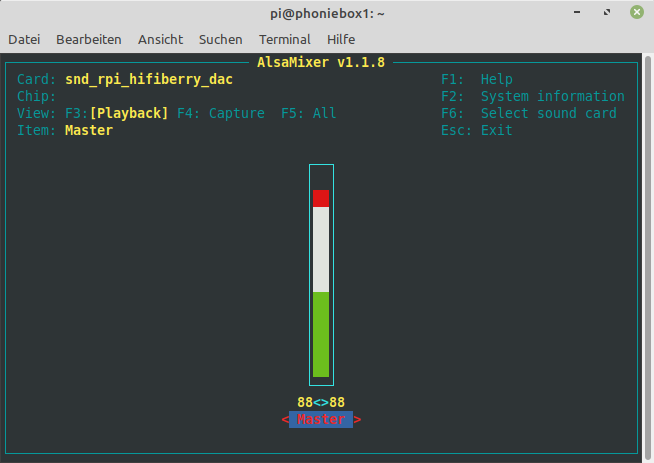
\includegraphics[width=0.9\textwidth]{software/alsamixer.png}
\caption{Lautst�rkeeinstellung mit dem \software{alsamixer}}
\label{fig:alsamixer}
\end{figure}

% chapter3_4.tex -- de (German)
% manual installation of the Phoniebox software
\newpage
\section{Manuelle Installation der \Bezeichnung-Software}

\begin{bclogo}[logo = \bclampe, noborder = true]{Hinweis}
Eigentlich sollte die Installation mit Hilfe des sogenannten
\software{one line installers} funktionieren. Mit etwas Gl�ck l�uft die
Installation problemlos durch, weil alle gemeldeten Fehler durch die
Projekt-Maintainer ausgemerzt wurden. Insbesondere Neulinge sollten
zuerst den \software{one line installer} ausprobieren, bevor sie sich an
den folgenden Einzelkommandos austoben \smiley{wink}\\
\begin{smaller}
\url{https://github.com/MiczFlor/RPi-Jukebox-RFID/wiki/INSTALL-stretch#one-line-install-command}
\end{smaller}
Bei Erfolg kann dieses Kapitel ggf. komplett �bersprungen werden.
\smiley{smile}
\end{bclogo}

Beim {\autor} lief es nat�rlich anders und er f�hrte dann unter 
\os{Raspbian Buster Lite} Anfang Januar 2020 die Installation der
\Bezeichnung-Soft\-ware manuell durch. Dabei traten diverse Probleme
auf, die bei den einzelnen Schritten beschrieben werden. Es kann
nat�rlich jederzeit sein, dass aufgrund von Aktualisierungen im
github-Re\-po\-si\-to\-ry sowohl der \software{one line installer} als
auch die Einzelkommandos wieder funktionieren\dots

Dieses Kapitel orientiert sich dabei an der Installationsanleitung auf
github ab dem Abschnitt \textit{install required packages and the
Phoniebox code}:\\
\begin{scriptsize}
\url{https://github.com/MiczFlor/RPi-Jukebox-RFID/wiki/INSTALL-stretch#install-required-packages-and-the-phoniebox-code}
\end{scriptsize}


\subsection{ben�tigte Programmpakete und -bibliotheken installieren}
\label{sect:apt-get}
F�r den Betrieb der \Bezeichnung-Soft\-ware sind etliche Programmpakete
erforderlich, die �ber \cmd{apt-get} installiert werden. Vor der
Installation empfiehlt es sich, zun�chst das Kommandopaar\\
\cmdPi{sudo apt-get update \&\& sudo apt-get upgrade}\\
abzusetzen, da sich gerade bei \os{Raspbian} in den Repositorys st�ndig
viel �ndert!

\cmdPi{sudo apt-get install apt-transport-https}\\
\cmdPi{sudo apt-get install samba samba-common-bin}
\comment{siehe Abfrage aus Abbildung \ref{fig:apt-get_samba}}\\
\cmdPi{sudo apt-get install python-dev python-pip}\\
\cmdPi{sudo apt-get install \textcolor{red}{python3-dev python3-pip}}
%\comment{Python3 kann hier auf keinen Fall schaden!}\\
\comment{Python3 ist hier kein Fehler!}\\
\cmdPi{sudo apt-get install gcc raspberrypi-kernel-headers lighttpd}\\
\cmdPi{sudo apt-get install php7.3-common php7.3-cgi php7.3 php7.3-fpm}\\
\cmdPi{sudo apt-get install at mpd mpc mpg123}\\
\cmdPi{sudo apt-get install git ffmpeg python-mutagen}\\
\cmdPi{sudo apt-get install \textcolor{red}{python3-mutagen}}
\comment{Python3 schadet auch hier auf keinen Fall!}

\begin{bclogo}[logo = \bclampe, noborder = true]{Hinweis}
In Kapitel \ref{sect:systemd} hat mich dann auch das Fehlen von Python3
eingeholt, weil in der Originalanleitung in Abschnitt \ref{sect:evdev}
nur die Python2-Version installiert wurde\dots \smiley{sarcastic}
\end{bclogo}

\begin{figure}[h]
\centering
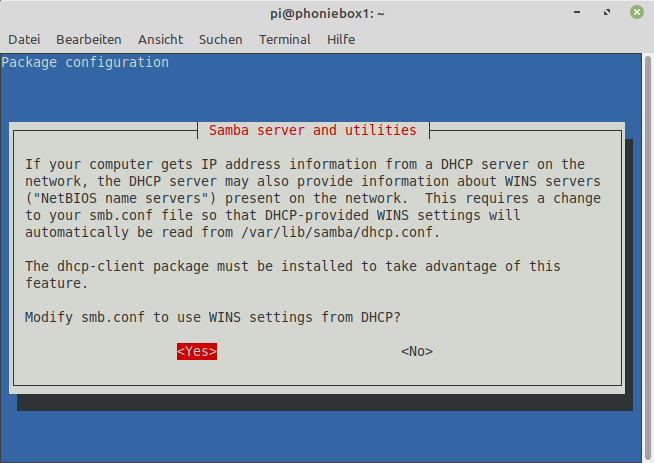
\includegraphics[width=0.88\textwidth, angle=0]{software/apt-get_samba.png}
\caption{Abfrage bei der Installation von \software{Samba} mit \cmd{apt-get}}
\label{fig:apt-get_samba}
\end{figure}

Bei der Installation von \software{Samba} erscheint die Abfrage aus
Abbildung \ref{fig:apt-get_samba}, die wie abgebildet mit \cmd{Yes}
beantwortet wird.
        

\subsection{Projekt \texttt{RPi-Jukebox-RFID} von \textit{github} klonen und installieren}
\cmdPi{git clone https://github.com/MiczFlor/RPi-Jukebox-RFID.git}\\
\cmdPi{cd RPi-Jukebox-RFID}

In der Datei requirements.txt ist (vermutlich au einem alten Stand
herr�hrend) das Paket spidev auskommentiert.

\cmdPi{nano requirements.txt}\\
\editor{\# Library dependencies for the python code.  You need to install these with\\
        \# `sudo pip install -r requirements.txt` before you can run this.\\
        \\
        \#\#\#\# ESSENTIAL LIBRARIES FOR MAIN FUNCTIONALITY \#\#\#\#\\
        \# related libraries.\\
        evdev==0.7.0\\
        git+git://github.com/lthiery/SPI-Py.git\#egg=spi-py\\
        youtube\_dl\\
        pyserial\\
%        \sout{\# spidev - currently installed via apt-get}\comment{eben nicht!}\\
%        \textcolor{blue}{\# added by schlizb�da:\\ spidev}\\
        \textcolor{red}{\# spidev - currently installed via apt-get}\comment{eben nicht!}\\
        RPi.GPIO\\
        pi-rc522
       }
       
\begin{bclogo}[arrondi = 0.2, logo = \bcinfo, ombre = true, epOmbre = 0.25, couleurOmbre = black!30,blur]{Achtung}
Im Gegensatz zum Kommentar in der roten Zeile wird das Paket
\software{spidev} nicht\\installiert. Dies f�hrt zu folgender
Fehlermeldung beim Kommando:\\
\cmdPi{pip install -r requirements.txt}
\end{bclogo}

\begin{smaller}
\begin{verbatim}
Looking in indexes: https://pypi.org/simple, https://www.piwheels.org/simple
Collecting evdev==0.7.0 (from -r requirements.txt (line 7))
  Downloading https://files.pythonhosted.org/packages/67/15/eac376f3e1fc1960a54439c21459b2582e68340001aff83b4ace9e5bd110/evdev-0.7.0.tar.gz
Collecting spi-py from git+git://github.com/lthiery/SPI-Py.git#egg=spi-py (from -r requirements.txt (line 8))
  Cloning git://github.com/lthiery/SPI-Py.git to /tmp/pip-install-uDNQOf/spi-py
Collecting youtube_dl (from -r requirements.txt (line 9))
  Downloading https://files.pythonhosted.org/packages/d0/b3/c3d42f6bbf91da104c272950d30923c222061d7323aa43dcf975a6e8e2c2/youtube_dl-2020.3.24-py2.py3-none-any.whl (1.8MB)
    100% |xxxxxxxxxxxxxxxxxxxxxxxxxxxxxxxx| 1.8MB 129kB/s 
Collecting pyserial (from -r requirements.txt (line 10))
  Downloading https://files.pythonhosted.org/packages/0d/e4/2a744dd9e3be04a0c0907414e2a01a7c88bb3915cbe3c8cc06e209f59c30/pyserial-3.4-py2.py3-none-any.whl (193kB)
    100% |xxxxxxxxxxxxxxxxxxxxxxxxxxxxxxxx| 194kB 608kB/s 
Requirement already satisfied: RPi.GPIO in /usr/lib/python2.7/dist-packages (from -r requirements.txt (line 12)) (0.7.0)
Collecting pi-rc522 (from -r requirements.txt (line 13))
  Downloading https://files.pythonhosted.org/packages/84/f2/e3d02257949e9caa9bff26044e0185e743ff45d3e0e099a93880e10bf718/pi-rc522-2.2.1.tar.gz
    Complete output from command python setup.py egg_info:
    Traceback (most recent call last):
      File "<string>", line 1, in <module>
      File "/tmp/pip-install-uDNQOf/pi-rc522/setup.py", line 11, in <module>
        from pirc522 import __version__  # flake8: noqa
      File "pirc522/__init__.py", line 4, in <module>
        from .rfid import RFID
      File "pirc522/rfid.py", line 2, in <module>
        import spidev
    ImportError: No module named spidev
\end{verbatim}
\textcolor{red}{Command "python setup.py egg\_info"\ failed with error code 1 in /tmp/pip-install-uDNQOf/pi-rc522/}
\end{smaller}

\textbf{Deshalb die Python-Software so installieren:}\\
\cmdPi{echo spidev >spidev.txt}\\
\cmdPi{pip install -r spidev.txt}\\
\cmdPi{pip install -r requirements.txt}

Hiermit l�uft die Python-Installation fehlerfrei durch!


\subsection{Einbinden des RFID-Lesers als Python(?)-Event}
\label{sect:evdev}
\cmdPi{pip install evdev}
\begin{smaller}
\begin{verbatim}
Looking in indexes: https://pypi.org/simple, https://www.piwheels.org/simple
Requirement already satisfied: evdev in /home/pi/.local/lib/python2.7/site-packages (0.7.0)
\end{verbatim}
\end{smaller}

\begin{bclogo}[logo = \bclampe, noborder = true]{Hinweis}
Aufgrund der obigen Meldung scheint das Python2-Paket \texttt{evdev}
bereits aktuell zu sein. \textcolor{red}{Viel wichtiger ist aber, dass
diese Bibliothek anschlie�end auch f�r \software{Python3} installiert
wird!}
\end{bclogo}

\cmdPi{pip3 install evdev}
\begin{smaller}
\begin{verbatim}
Looking in indexes: https://pypi.org/simple, https://www.piwheels.org/simple
Collecting evdev
  Downloading https://www.piwheels.org/simple/evdev/evdev-1.3.0-cp37-cp37m-linux_armv7l.whl (98kB)
    100% |xxxxxxxxxxxxxxxxxxxxxxxxxxxxxxxx| 102kB 628kB/s 
Installing collected packages: evdev
Successfully installed evdev-1.3.0
\end{verbatim}
\end{smaller}


\subsection{Webserver \software{lighttpd} f�r die Web-App der {\Bezeichnung} einrichten}
Auch bei der Web-App l�uft's ganz und gar nicht wie geschmiert.
\smiley{nosmile}

\textbf{Datei \filenam{/etc/lighttpd/lighttpd.conf} bearbeiten}\\
In der Datei \filenam{/etc/lighttpd/lighttpd.conf} m�ssen folgende
�nderungen (rot) erg�nzt werden:\\
\cmdPi{sudo nano /etc/lighttpd/lighttpd.conf}\\
\editor{\textcolor{red}{\# adjusted by schlizb�da due to https://github.com/MiczFlor/RPi-Jukebox-RFID/wiki/INSTALL-stretch\#lighttpd-web-server-for-web-app\\
server.document-root        = "/home/pi/RPi-Jukebox-RFID/htdocs"\\
\#}server.document-root        = "/var/www/html"\\
server.upload-dirs          = ( "/var/cache/lighttpd/uploads" )\\
server.errorlog             = "/var/log/lighttpd/error.log"\\
server.pid-file             = "/var/run/lighttpd.pid"\\
server.username             = "www-data"\\
server.groupname            = "www-data"\\
server.port                 = 80
}

\textbf{Datei \filenam{/etc/sudoers} bearbeiten}\\
Hier muss hinten der rot eingef�rbte Teil angeh�ngt werden:\\
\editor{\#\\
\# This file MUST be edited with the 'visudo' command as root.\\
\#\\
\# Please consider adding local content in /etc/sudoers.d/ instead of\\
\# directly modifying this file.\\
\#\\
\# See the man page for details on how to write a sudoers file.\\
\#\\
Defaults        env\_reset\\
Defaults        mail\_badpass\\
Defaults        secure\_path="/usr/local/sbin:/usr/local/bin:/usr/sbin:/usr/bin:/sbin:/bin"
}
%\\
%\# Host alias specification\\
%\\
%\# User alias specification\\
%\\
%\# Cmnd alias specification\\
%\\
%\# User privilege specification\\
%root    ALL=(ALL:ALL) ALL\\
%\\
%\# Allow members of group sudo to execute any command\\
%%sudo   ALL=(ALL:ALL) ALL\\
%\\
%\# See sudoers(5) for more information on "\#include" directives:\\
%\\
%\#includedir /etc/sudoers.d\\
%\\
\texttt{\\
\begin{small}%\textcolor{gray}{\vdots}\\
    \textcolor{red}{\textit{\# added by schlizb�da:\\www-data ALL=(ALL) NOPASSWD: ALL}}
    \\\textcolor{gray}{\vdots}
\end{small}}

\textbf{Modul \texttt{fastcgi} f�r den Webserver \software{lighttpd} konfigurieren}\\
Damit der Webserver die bei der {\Bezeichnung} zum Einsatz kommenden
HP-Scrip\-te ausf�hren kann, muss das Modul \texttt{fastcgi} mit den
folgenden Kommandos einmalig aktiviert werden:\\
\cmdPi{sudo lighttpd-enable-mod fastcgi}\\
\stdout{Enabling fastcgi: ok\\
        Run "{}service lighttpd force-reload"\ to enable changes}\\
\cmdPi{sudo lighttpd-enable-mod fastcgi-php}\\
\stdout{Enabling fastcgi-php: ok\\
        Run "{}service lighttpd force-reload" to enable changes}

%M�glicherweise ist die Konfiguration noch auf PHP5 eingestellt. F�r die
%{\Bezeichnung} wird aber PHP7 ben�tigt. Daher muss die Datei
%\filenam{/etc/lighttpd/conf-available/15-fastcgi-php.conf} angepasst
%werden.
%\begin{bclogo}[arrondi = 0.2, logo = \bcinfo, ombre = true, epOmbre = 0.25, couleurOmbre = black!30,blur]{Achtung}
%Unter \os{Raspbian Buster} kommt mittlerweile \textcolor{red}{PHP7.3}
%zum Einsatz, nicht mehr PHP7.0! Von daher muss beim Editieren auch die
%richtige Versionsnummer eingetragen werden.\\
%Auch dies wurde in der Anleitung unter\\
%\begin{scriptsize}\url{https://github.com/MiczFlor/RPi-Jukebox-RFID/wiki/INSTALL-stretch#lighttpd-web-server-for-web-app}\end{scriptsize}\\
%noch nicht ber�cksichtigt und angepasst!
%\end{bclogo}
%\cmdPi{sudo nano /etc/lighttpd/conf-available/15-fastcgi-php.conf}\\
%\editor{\# -*- depends: fastcgi -*-\\
%\# /usr/share/doc/lighttpd/fastcgi.txt.gz\\
%\# http://redmine.lighttpd.net/projects/lighttpd/wiki/Docs:ConfigurationOptions\#mod\_fastcgi-fastcgi\\
%\\
%\#\# Start an FastCGI server for php (needs the php5-cgi package)\\
%fastcgi.server += ( ".php" =>\\
%\tab[1cm]((\\
%\tab[2cm]"{}socket" => "/var/run/php/\textcolor{red}{php7.3-fpm.sock}",\\
%\tab[2cm]"broken-scriptfilename" => "{}enable"\\
%\tab[1cm]))
%)}

Die neue Konfiguration des \software{lighttpd}-Webservers neu laden:\\
\cmdPi{sudo service lighttpd force-reload}


\textbf{Upload von Audiodateien �ber den Webservice erm�glichen}\\
Um den Webservice f�r den Upload von Audiodateien auf die {\Bezeichnung}
zu ert�chtigen, muss die Datei \filenam{/etc/php/7.3/fpm/php.ini}
angelegt werden. Dazu ist im github-Repository der {\Bezeichnung} eine
Beispieldatei vorhanden:\\
\cmdPi{\begin{scriptsize}sudo cp /home/pi/RPi-Jukebox-RFID/misc/sampleconfigs/php.ini.stretch-default.sample /etc/php/\textcolor{red}{7.3}/fpm/php.ini\end{scriptsize}}
\cmdPi{sudo chown root:root /etc/php/\textcolor{red}{7.3}/fpm/php.ini}\\
\cmdPi{sudo chmod 644 /etc/php/\textcolor{red}{7.3}/fpm/php.ini}

In der Datei \texttt{/etc/php/7.3/fpm/php.ini} sind folgende Eintr�ge zu
kontrollieren und gegebenenfalls zu erg�nzen:\\
\cmdPi{sudo nano /etc/php/\textcolor{red}{7.3}/fpm/php.ini}\\
\editor{file\_uploads = On\\
upload\_max\_filesize = 0\\
max\_file\_uploads = 20\\
post\_max\_size = 0
}

\cmdPi{sudo service \textcolor{red}{php7.3-fpm} restart}


\textbf{Konfigurationsdatei f�r die Web-App aus der Beispieldatei kopieren}\\
\cmdPi{\begin{smaller}cp /home/pi/RPi-Jukebox-RFID/htdocs/config.php.sample /home/pi/RPi-Jukebox-RFID/config.php\end{smaller}}

\textbf{Zugriff auf Verzeichnisse \filenam{shared} und \filenam{htdocs} f�r den Webservice erm�glichen}\\
Der Zugriff erfolgt unter dem Benutzer \texttt{www-data}, daher muss der
Zugriff auf die beiden Verzeichnisse f�r diesen Benutzer �ber
Gruppenrechte erm�glicht werden:\\
\cmdPi{sudo chown -R pi:www-data /home/pi/RPi-Jukebox-RFID/shared}\\
\cmdPi{sudo chmod -R 775 /home/pi/RPi-Jukebox-RFID/shared}\\
\cmdPi{sudo chown -R pi:www-data /home/pi/RPi-Jukebox-RFID/htdocs}\\
\cmdPi{sudo chmod -R 775 /home/pi/RPi-Jukebox-RFID/htdocs}


\newpage
\textbf{Kontrolle im Browser:}\\
\begin{figure}[!h]
\centering
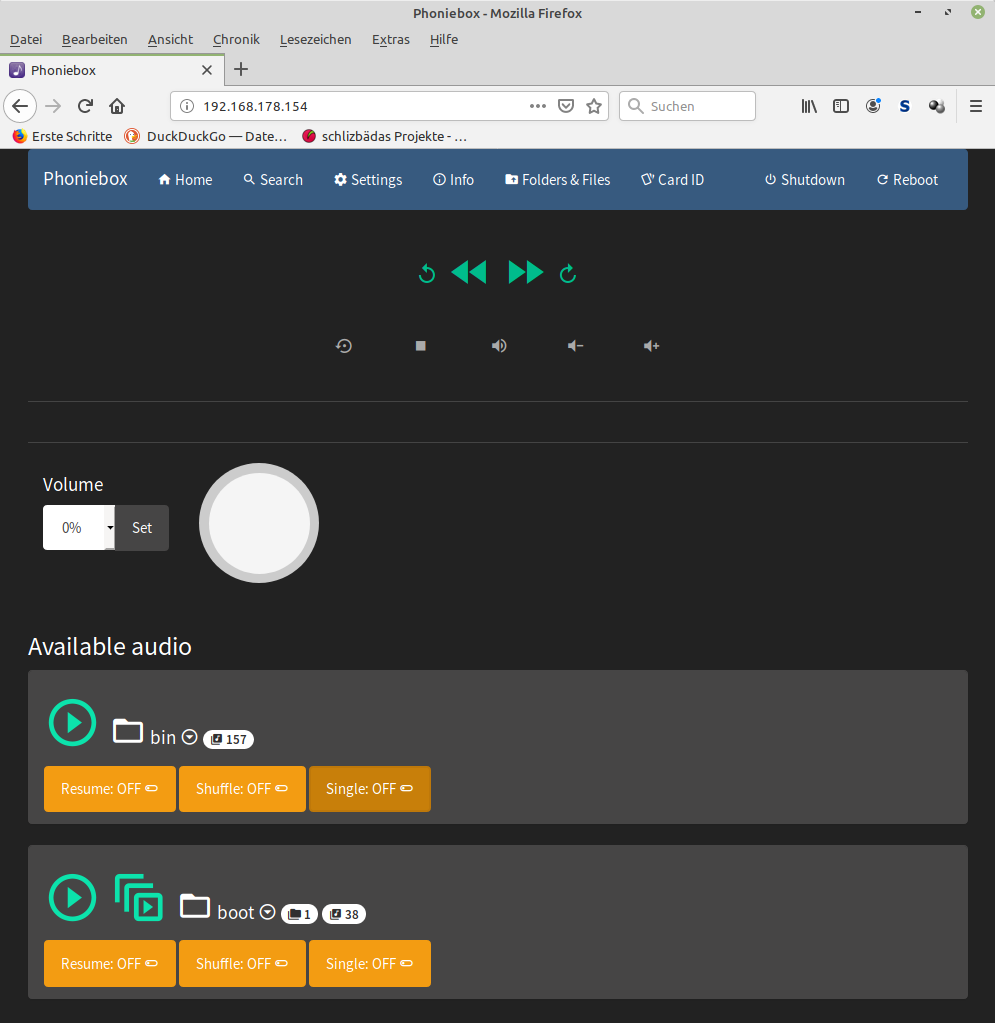
\includegraphics[width=1\textwidth, angle=0]{software/lighttpd_webserver.png}
\caption{Aufruf des \software{lighttpd}-Webservers}
\label{fig:lighttpd_webserver}
\end{figure}

Hintergrunddetails zur Einrichtung des Webservers siehe:\\
\begin{smaller}
\url{https://github.com/MiczFlor/RPi-Jukebox-RFID/wiki/INSTALL-stretch#lighttpd-web-server-for-web-app}
\end{smaller}

% chapter3_5.tex -- de (German)
% configuration of mpd
\newpage
\section{\software{Music Player Daemon (mpd)} einrichten}
Die gesamte Konfiguration des \software{mpd} wird in der Datei
\filenam{/etc/mpd.conf} vorgenommen. Diese Datei besteht aus Eintr�gen
in der Form \textit{Schl�sselwort Wert} und in der Standardauslieferung
aus vielen Kommentarzeilen. Letztlich m�ssen folgende Eintr�ge erg�nzt
oder angepasst werden:\\
\cmdPi{sudo nano /etc/mpd.conf}\\
\editor{music\_directory    "{}/home/pi/RPi-Jukebox-RFID/shared/audiofolders"\\
playlist\_directory "{}/home/pi/RPi-Jukebox-RFID/playlists"\\
user               "root"\\
auto\_update        "yes"\\ % (you have to remove the \# in front of that line)\\
auto\_update\_depth  "10"\\ % (remove the \# and change the value to 10)\\
%\#mixer\_control      "yourAudioIfaceNameHere"\\ % (you need to uncomment this line and change the audio iFace shortname)\\
mixer\_control      "Master"
}
        
Folgendes Kommando dient dazu, die Bezeichnung f�r den Eintrag
\texttt{mixer\_control} herauszufinden:\\
\cmdPi{amixer scontrols}\comment{liefert z.B. bei \miniamp-Installation}\\
\stdout{Simple mixer control 'Master',0}

Der \software{mpd} wird mit der neuen Konfiguration mit folgendem
Kommando gestartet:\\
\cmdPi{mpc update}

\textbf{Test von \software{mpd}}\\
Jetzt ist der Zeitpunkt gekommen, einen geschmeidigen Audiotest mit
\software{mpd} durchzuf�hren. Dazu zun�chst vom PC eine Audiodatei
auf den {\RPi} in das oben konfigurierte Audioverzeichnis
\filenam{/home/pi/RPi-Jukebox-RFID/shared/audiofolders} kopieren und
mit dem Client \software{mpc} abspielen:\\
\cmdPC{scp /Pfad/Musik.flac pi@phoniebox1:/home/pi/RPi-Jukebox-RFID/shared/audiofolders}

\cmdPi{mpc add /home/pi/RPi-Jukebox-RFID/shared/audiofolders/Musik.flac}\\
\cmdPi{mpc play}

Sollte keine Musik h�rbar sein, mit dem \software{alsamixer} die
Lautst�rke �berpr�fen und anpassen:\\
\cmdPi{alsamixer}

(siehe Abbildung \ref{fig:alsamixer})


% chapter3_6.tex -- de (German)
% installation of the RFID reader
\newpage
%\begin{bclogo}[logo = \bclampe, noborder = true]{Hinweis}
\begin{bclogo}[arrondi = 0.2, logo = \bcinfo, ombre = true, epOmbre = 0.25, couleurOmbre = black!30,blur]{Achtung}
Ab hier bezieht sich diese Dokumentation auf die Seite\\
\url{https://github.com/MiczFlor/RPi-Jukebox-RFID/wiki/CONFIGURE-stretch}\\
von MiczFlor!
\end{bclogo}

\section{{\reader} installieren}
In diesem Abschnitt wird die Installation des \textit{Neuftech USB
RFID-Reader 125kHz} beschrieben, der in {\autor}s {\Bezeichnung}
verbaut wurde und bei amazon erh�ltlich ist:\\
\url{https://www.amazon.de/Neuftech-Reader-Kartenleseger%C3%A4t-Kartenleser-Kontaktlos/dp/B018OYOR3E}

Dieses Ger�t emuliert am USB-Anschluss eine Tastatur (ein Ger�t aus der
USB-Klasse \textit{Human Interface Device},
\url{https://de.wikipedia.org/wiki/Human_Interface_Device}).\\
Die \Bezeichnung-Soft\-ware f�ngt Ereignisse vom {\reader} jedoch �ber
\software{udev} ab:\\
\url{https://wiki.ubuntuusers.de/udev/}


\subsection{{\reader} �berpr�fen}
Einen unter \os{Raspbian} korrekt installierten {\reader} erkennt man
durch Kontrolle folgender Punkte
\begin{compactitem}
\item{Die LED des {\reader}s leuchtet -- im eingebauten Zustand evtl. nicht erkennbar}
\item{Piepton beim Hochfahren}
\item{Piepton beim Lesen einer \Karte}
\item{�berpr�fen, ob das Softwareevent f�r den {\reader} ordnungsgem��
      eingerichtet ist:\\
      \cmdPi{ls -la /dev/input/by-id}\\
      \stdout{total 0\\
              drwxr-xr-x 2 root root  60 Jan 11 15:36 .\\
              drwxr-xr-x 4 root root 120 Jan 11 15:36 ..\\
              lrwxrwxrwx 1 root root   9 Jan 11 15:36 usb-HXGCoLtd\_27db-event-kbd -> ../event0}
     }
\end{compactitem}


\subsection{{\reader} in der \Bezeichnung-Software registrieren}
\cmdPi{cd /home/pi/RPi-Jukebox-RFID/scripts}\\
\cmdPi{python2 RegisterDevice.py}\comment{liefert \zB:}\\
\stdout{Choose the reader from list\\
0 HID 046a:0011\\
\textcolor{red}{1 HXGCoLtd Keyboard}\\
Device Number: \textbf{\textcolor{red}{1}}}\\
Unter Linux wird der Chipsatz des {\reader}s als \textit{HXGCoLtd
Keyboard} erkannt. Daher ist bei der Abfrage der \texttt{Device Number}
in diesem Beispiel der Wert \textcolor{red}{1} einzugeben.

Ob die Registrierung des {\reader}s erfolgreich war, kann mit der Datei\\
\filenam{/home/pi/RPi-Jukebox-RFID/scripts/deviceName.txt} gepr�ft
werden. Diese Datei enth�lt den oben gew�hlten Ger�tenamen:\\
\cmdPi{cat deviceName.txt}\\
\stdout{HXGCoLtd Keyboard}


\subsection{RFID-Konfigurationsdatei der \Bezeichnung-Software anlegen}
\cmdPi{cd /home/pi/RPi-Jukebox-RFID/settings}\\
\cmdPi{cp rfid\_trigger\_play.conf.sample rfid\_trigger\_play.conf}\\
\cmdPi{sudo chown pi:pi rfid\_trigger\_play.conf}\\ % braucht's das?
\cmdPi{sudo chmod 665 rfid\_trigger\_play.conf}     % braucht's das?













% chapter3_7.tex -- de (German)
% audio parameters
\section{Konfigurationsdateien im Verzeichnis \filenam{RPi-Jukebox-RFID/settings}}
%%%%\section{Audioparameter der {\Bezeichnung} setzen}
Das Unterverzeichnis filenam{/home/pi/RPi-Jukebox-RFID/settings} enth�lt
einige Konfigurationsdateien, in denen das Verhalten der {\Bezeichnung}
eingestellt und angepasst werden kann. Der Dateiinhalt bestaht dabei nur
aus dem gew�nschten Parameter. Die Funktion wird durch den Dateinamen
bestimmt und ist in den jeweiligen Python- \bzw Shellskripten fest
hinterlegt.\\
siehe\\
\begin{smaller}\url{https://github.com/MiczFlor/RPi-Jukebox-RFID/wiki/CONFIGURE-stretch#create-settings-for-audio-playout}\end{smaller}

\subsection{Audioeinstellungen}
Die folgenden Kommandos legen im Verzeichnis
\filenam{/home/pi/RPi-Jukebox-RFID/settings} kleine Textdateien an, die
das Verhalten der Taster \textit{volume up} und \textit{volume down}
konfigurieren. Ferner kann die maximale Lautst�rke begenzt werden:\\
\cmdPi{echo "Master"{} > /home/pi/RPi-Jukebox-RFID/settings/Audio\_iFace\_Name}\\
\cmdPi{echo "3"{} > /home/pi/RPi-Jukebox-RFID/settings/Audio\_Volume\_Change\_Step}\\
\cmdPi{echo "100"{} > /home/pi/RPi-Jukebox-RFID/settings/Max\_Volume\_Limit}

MP3-Dateien f�r Startup und Shutdown kopieren:\\
\cmdPi{\begin{scriptsize}cp /home/pi/RPi-Jukebox-RFID/misc/sampleconfigs/startupsound.mp3.sample\\ /home/pi/RPi-Jukebox-RFID/shared/startupsound.mp3\end{scriptsize}}\\
\cmdPi{\begin{scriptsize}cp /home/pi/RPi-Jukebox-RFID/misc/sampleconfigs/shutdownsound.mp3.sample\\ /home/pi/RPi-Jukebox-RFID/shared/shutdownsound.mp3\end{scriptsize}}

\subsection{automatische Abschaltung bei Nichtbenutzung}
Gerade bei Kindern ist es sinnvoll, die {\Bezeichnung} nach einiger Zeit
der Nichtverwendung automatisch abzuschalten, um die Akkulaufzeit zu
verl�ngern. Der angegebene Wert ist inaktive Zeit in Minuten
\textit{ab dem Beenden der \software{mpd}-Playlist}, bevor sich die Box
automatisch abschaltet. Der Wert 0 deaktiviert diese Funktion.\\ 
\cmdPi{echo "0"{} > /home/pi/RPi-Jukebox-RFID/settings/Idle\_Time\_Before\_Shutdown}

Ein automatisches Abschalten der {\Bezeichnung} nach 15 Minuten
Nichtbenutzung erreicht man alternativ durch:\\
\cmdPi{echo "15"{} > /home/pi/RPi-Jukebox-RFID/settings/Idle\_Time\_Before\_Shutdown}%\comment{Alternative}


% chapter3_08.tex -- de (German)
% Using GPIO hardware buttons
\section{Die {\Bezeichnung} mit Tastern an der GPIO-Leiste steuern}
\label{sect:GPIO-buttons}

Urspr�nglich war vorgesehen, bestimmte {\Karte}n mit
Steuerungsfunktionen zu belegen. Dieses Konzept ist aber gerade bei
Kindern ung�nstig, da (zumindest meine) Kinder solche Sachen in den
Tiefen ihrer Zimmer sehr gut verstecken \smiley{smile} und die
{\Bezeichnung} damit zwischenzeitlich(?) unbedienbar wird.\\ 
Daher hat MiczFlor in seinem github-Repository das Kapitel
\url{https://github.com/MiczFlor/RPi-Jukebox-RFID/wiki/Using-GPIO-hardware-buttons}
eingef�gt, in dem die Inbetriebnahme der Steuerung �ber Taster an der
GPIO-Leiste beschrieben wird.

\begin{bclogo}[arrondi = 0.2, logo = \bcinfo, ombre = true, epOmbre = 0.25, couleurOmbre = black!30,blur]{Achtung}
Die Pinbelegung in der Anleitung von MiczFlor ordnet den Tastern Pins
zu, die f�r die digitale Audio�bertragung �ber I2S zum HifiBerry
{\miniamp} ben�tigt werden! Daher muss das Pythonskript f�r die
Abfrage der Taster stark angepasst werden!
\end{bclogo}

F�r den Zugriff auf die GPIOs wird die Python-Bibliothek
\software{gpiozero} verwendet, von der es jeweils eine eigene Variante
f�r Python2 und Python 3 gibt. Installation der Bibliothek �ber
folgendes Kommando:\\
\cmdPi{sudo apt-get install python3-gpiozero python-gpiozero}
\comment{f�r Python2 \textbf{und} 3!}

Zur Abfrage der Taster wird das Pythonskript
\filenam{/home/pi/RPi-Jukebox-RFID/scripts/gpio-buttons.py} verwendet.
Die Originalvorlage k�nnte mit folgendem Kommando installiert werden:\\
\cmdPi{\begin{scriptsize}sudo cp /home/pi/RPi-Jukebox-RFID/misc/sampleconfigs/gpio-buttons.py.sample\\ /home/pi/RPi-Jukebox-RFID/scripts/gpio-buttons.py\end{scriptsize}}
\comment{funktioniert nicht mit dem \miniamp!}\\
Allerdings kollidiert die Pinvergabe mit der Pinzuordnung des HifiBerry
{\miniamp}s!

Bei Einbau des {\miniamp}s muss die von {\autor} angepasste Datei
verwendet werden! Diese Datei entspricht der Pinbelegung der
Lochrasterplatine aus Kapitel \ref{sect:prototypingboard}:\\
\cmdPC{scp ./files/GPIO/gpio-buttons.py pi@phoniebox1:/home/pi/RPi-Jukebox-RFID/scripts}

\cmdPi{nano /home/pi/RPi-Jukebox-RFID/scripts/gpio-buttons.py}\\
%\begin{verbatim}
\verb|#shut = Button(3,hold_time=2)  # --> Pin 5 # no longer necessary due to OnOffShim|\\
\verb|vol0 = Button(13,pull_up=True) # --> Pin 33|\\
\verb|volU = Button(12,pull_up=True,hold_time=0.3,hold_repeat=True) # --> Pin 32|\\
\verb|volD = Button(6,pull_up=True,hold_time=0.3,hold_repeat=True)  # --> Pin 31|\\
\verb|next = Button(7,pull_up=True)  # --> Pin 26|\\
\verb|prev = Button(8,pull_up=True)  # --> Pin 24|\\
\verb|halt = Button(5,pull_up=True)  # --> Pin 29|\\
\verb|#reco = Button(6, pull_up=True) # Choose GPIO to fit your hardware|\\
\verb|#play = Button(12,pull_up=True) # Choose GPIO to fit your hardware|
%\end{verbatim}

siehe auch Tabelle \ref{tab:gpio_rpi}

% chapter3_9.tex -- de (German)
% assigning RFID cards to audio files/folders
\section{Zuordnung von H�rspielen zu {\Karte}n }
\label{sect:assignment}

\begin{bclogo}[logo = \bclampe, noborder = true]{Hinweis}
Die funktionalen Elemente der {\Bezeichnung} sind nun installiert. Jetzt
ist es an der Zeit, einzelnen H�rspielen oder Musikst�cken {\Karte}n
zuzuordnen und einen \textit{Soundcheck} zu machen, um die grundlegende
Funktionalit�t der Box zu �berpr�fen:
\end{bclogo}

\begin{figure}[!h]
\centering

\includegraphics[width=0.45\textwidth]{/software/helloween.jpg}

\includegraphics[width=0.45\textwidth]{/software/metallica.jpg}
\caption{Audiodaten (Musikalben) auf die {\Bezeichnung} kopieren}
\end{figure}

Zun�chst werden \textit{rekursiv} zwei Unterverzeichnisse mit den
Musikdateien zweier Musikalben vom PC in den Audioordner auf der 
{\Bezeichnung} kopiert:\\
\cmdPC{scp -r Helloween pi@phoniebox1:/home/pi/RPi-Jukebox-RFID/shared/audiofolders}\\
\cmdPC{scp -r Metallica pi@phoniebox1:/home/pi/RPi-Jukebox-RFID/shared/audiofolders}

Kontrolle mit \cmd{ls -lR} auf der {\Bezeichnung}:\\
\cmdPi{ls -lR /home/pi/RPi-Jukebox-RFID/shared/audiofolders}
\begin{smaller}
\begin{verbatim}
total 26728
drwxr-xr-x 2 pi pi           4096 May 17 15:50  Helloween
drwxr-xr-x 2 pi pi           4096 May 17 15:56  Metallica

./Helloween:
total 104140
-rwxr-xr-x 1 pi pi 37314544 May 17 15:47 01_I_Want_Out.flac
-rwxr-xr-x 1 pi pi 38112711 May 17 15:48 02_Dr._Stein.flac
-rwxr-xr-x 1 pi pi 31203347 May 17 15:49 03_Future_World.flac

./Metallica:
total 151828
-rwxr-xr-x 1 pi pi 38978523 May 17 15:52 01_Enter_Sandman.flac
-rwxr-xr-x 1 pi pi 41647915 May 17 15:54 02_Sad_But_True.flac
-rwxr-xr-x 1 pi pi 29319722 May 17 15:54 03_Holier_Than_Thou.flac
-rwxr-xr-x 1 pi pi 45518619 May 17 15:56 04_The_Unforgiven.flac
\end{verbatim}
\end{smaller}

\subsection{{\Karte} manuell zuordnen}
Um nun diesen beiden Alben zwei neue {\Karte}n zuzuordnen, sind folgende
Schritte erforderlich:
\begin{compactitem}
\item{ID der neuen {\Karte} herausfinden}
\item{F�r jede ID die Shortcut-Datei nacheditieren.} 
%\item{Playlist als \cmd{*.m3u}-Datei erstellen} # braucht's nicht!
%%%%
%\item{F�r jede ID die Shortcut-Datei \filenam{/home/pi/RPi-Jukebox-RFID/shared/shortcuts/000???????} anlegen, in der der Name einer \cmd{*.m3u}-Datei eingetragen ist.} 
%\item{Im Verzeichnis \filenam{/home/pi/RPi-Jukebox-RFID/playlists} die \cmd{*.m3u}-Datei mit dem oben angegebenen Namen anlegen}
\end{compactitem}

Zun�chst wird eine neue {\Karte} �ber den {\reader} eingelesen. Dabei
wird im Unterverzeichnis \filenam{/home/pi/RPi-Jukebox-RFID/shared/shortcuts}
eine Datei angelegt, die den Namen der Karten-ID hat, \zB \cmd{0009563230}.
Der Inhalt dieser Datei muss auf den Verzeichnisnamen des Albums oder
H�rbuchs unter \filenam{/home/pi/RPi-Jukebox-RFID/shared/audiofolders}
angepasst werden, \zB "`Helloween"'.\\
\cmdPi{nano /home/pi/RPi-Jukebox-RFID/shared/shortcuts/0009563230}\\
\stdout{Helloween}

%\subsection{ID einer neuen {\Karte} ermitteln}
%Die ID einer {\Karte} wird beim Einlesen durch den {\reader} in der
%Datei \filenam{/home/pi/RPi-Jukebox-RFID/settings/Latest\_RFID} abgelegt.
%Nach erfolgtem Einlesen den Inhalt dieser Datei anzeigen:\\
%\cmdPi{cat /home/pi/RPi-Jukebox-RFID/settings/Latest\_RFID}\\
%\stdout{0009563230}
%
%\subsection{Shortcut-Datei f�r die soeben ermittelte ID anlegen}
%Im Unterverzeichnis \filenam{/home/pi/RPi-Jukebox-RFID/shared/shortcuts}
%wird eine Datei angelegt, deren Dateiname der ermittelten ID, \zB 
%\cmd{0009563230} entspricht. In dieser Datei wird der Name des
%Unterverzeichnisses des gew�nschten Albums in\\
%\filenam{/home/pi/RPi-Jukebox-RFID/shared/audiofolders} eingetragen, \zB
%"`Helloween"'.\\
%\cmdPi{nano /home/pi/RPi-Jukebox-RFID/shared/shortcuts/0009563230}\\
%\stdout{Helloween}
%
%\subsection{Playlist f�r dieses Album als \cmd{*.m3u}-Datei erstellen}
%Die Playlist, die bei Auflegen dieser Karte abgespielt werden soll,
%muss im Verzeichnis\\ \filenam{/home/pi/RPi-Jukebox-RFID/playlists} als
%\cmd{*.m3u}-Datei erstellt werden. Dabei handelt es sich einfachsten
%Fall um eine Textdatei, die in jeder Zeile eine abzuspielende Audiodatei
%enth�lt, siehe \url{https://de.wikipedia.org/wiki/M3U}:\\
%\cmdPi{nano /home/pi/RPi-Jukebox-RFID/playlists/Helloween.m3u}\\
%\stdout{/home/pi/RPi-Jukebox-RFID/shared/audiofolders/Helloween/01\_I\_Want\_Out.flac\\
%        /home/pi/RPi-Jukebox-RFID/shared/audiofolders/Helloween/02\_Dr.\_Stein.flac\\
%        /home/pi/RPi-Jukebox-RFID/shared/audiofolders/Helloween/03\_Future\_World.flac
%       }

Nach erneutem Auflegen der {\Karte} mit der ID \cmd{0009563230} werden
%die in der Playlist hinterlegten Musiktitel des Albums \textit{Helloween
%-- The Best, The Rest, The Rare} abgespielt.
die im Verzeichnis \filenam{/home/pi/RPi-Jukebox-RFID/shared/audiofolders/Helloween}
abgelegten Audiodateien abgespielt.

%\begin{bclogo}[logo = \bclampe, noborder = true]{Hinweis}
%Wichtig ist bei diesem Vorgehen, dass sowohl der Dateiname der
%Playlist als auch das Albumsverzeichnis genau der Bezeichnung aus der
%Shortcut-Datei entsprechen muss, hier also "`Helloween"'!
%\end{bclogo}

\subsection{{\Karte} �ber die Webanwendung registrieren}
Alternativ kann eine {\Karte} auch mit Hilfe des Webservices zugeordnet
werden. Das Vorgehen wird in der folgenden Bilderstrecke dargestellt:

\begin{figure}[!h]
\centering
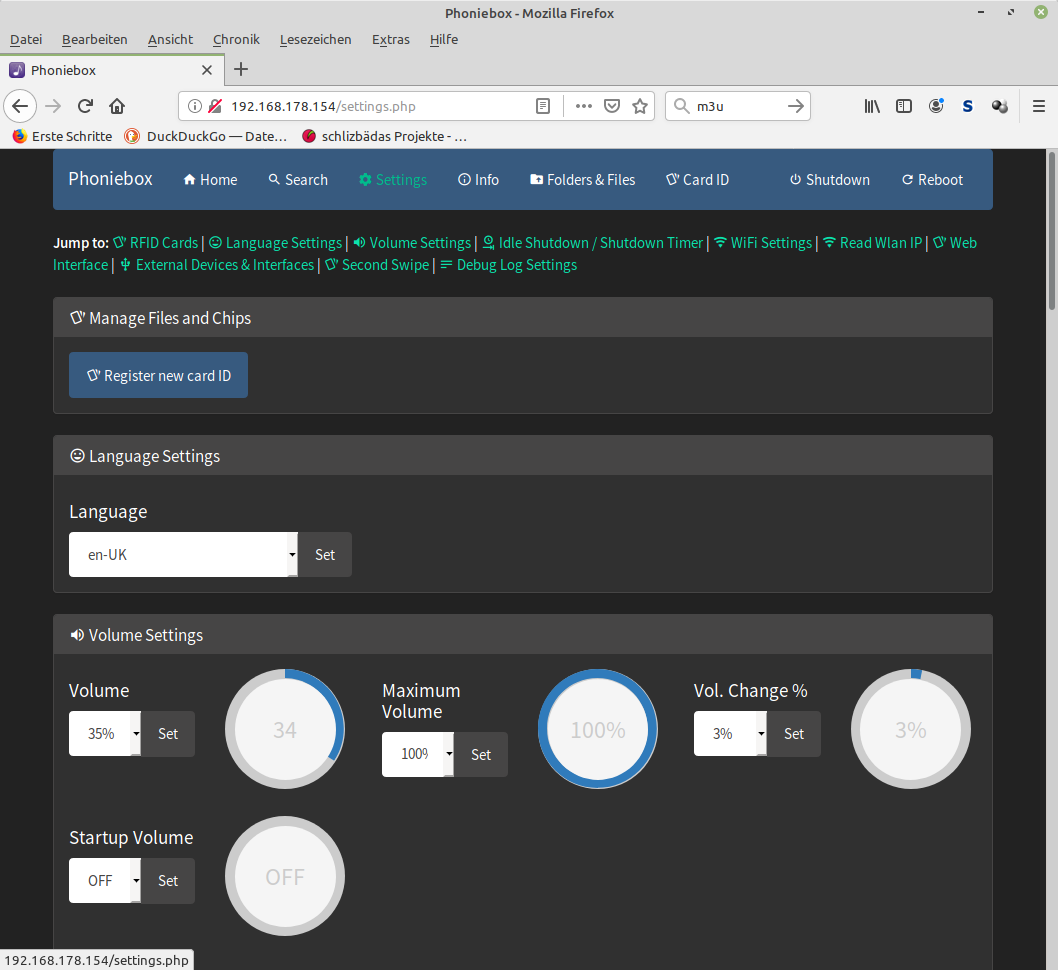
\includegraphics[width=0.49\textwidth]{/software/webservice-metallica01.png}
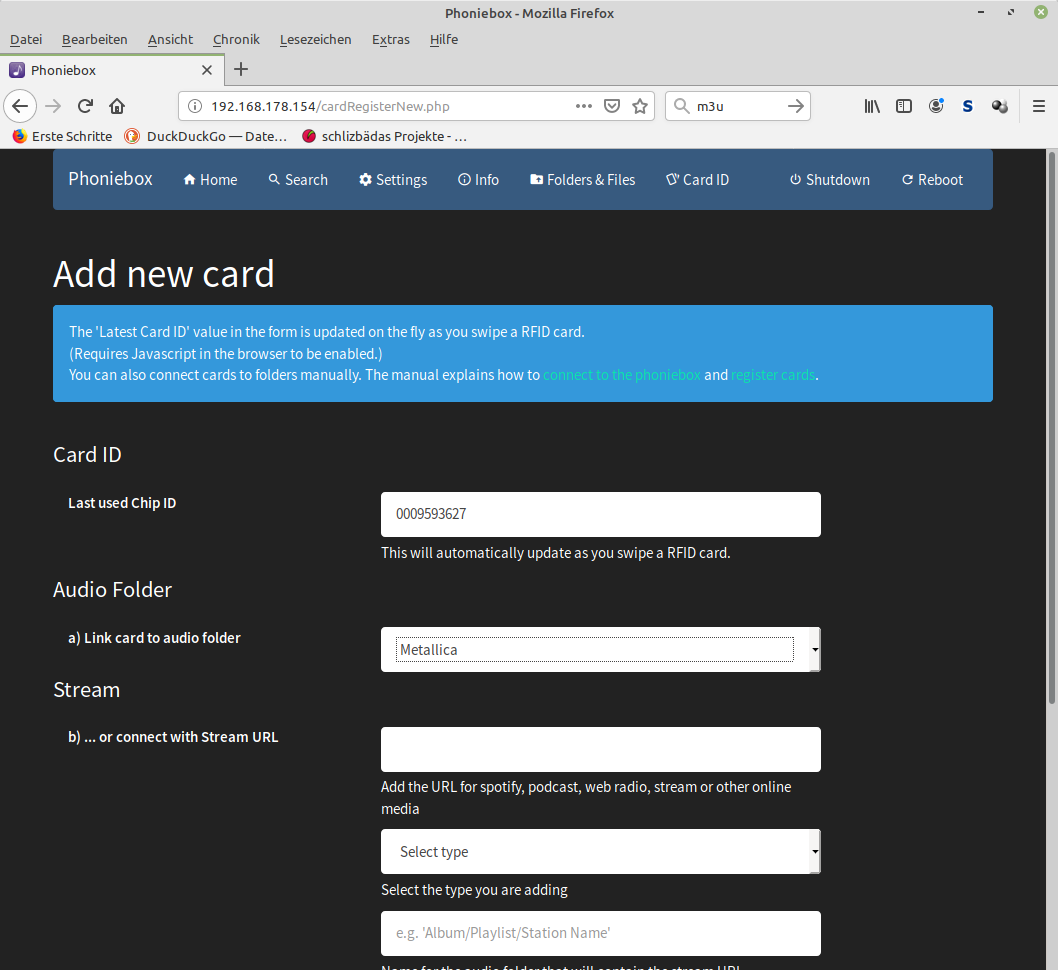
\includegraphics[width=0.49\textwidth]{/software/webservice-metallica02.png}
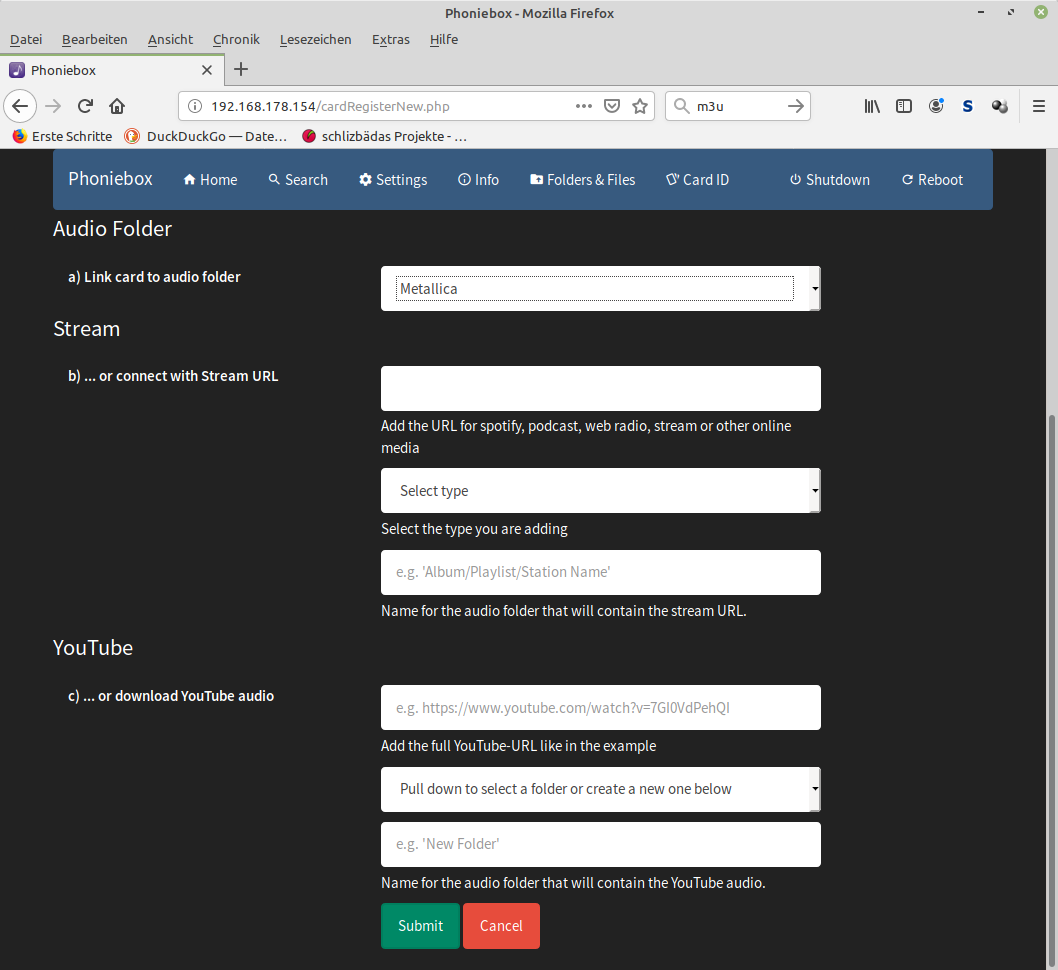
\includegraphics[width=0.49\textwidth]{/software/webservice-metallica03.png}
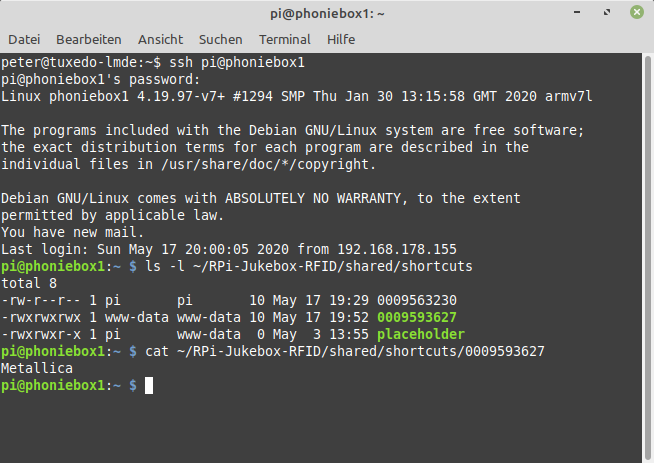
\includegraphics[width=0.49\textwidth]{/software/webservice-metallica04.png}
\caption{{\Karte} �ber Webservice registrieren}
\end{figure}

Am PC wird �ber einen Internetbrowser (Firefox) eine Verbindung zur
{\Bezeichnung} hergestellt, z.B. durch Eingabe der IP-Adresse (hier
192.168.178.154). Durch Klick auf \menuitem{Settings} in der oberen
Men�leiste erscheint das Bild links oben. Hier muss auf die Schaltfl�che
\button{Register new card ID} geklickt werden. Nun erscheint das Bild
rechts oben. Jetzt die neue {\Karte} �ber den {\reader} einlesen. Im
dazugeh�rigen Textfeld wird die ID aktualisiert (hier \cmd{0009593627}).

In der Zeile \menuitem{Audio Folder} werden im Auswahlfeld (ComboBox)
alle Unterverzeichnisse von \filenam{/home/pi/RPi-Jukebox-RFID/shared/audiofolders}
angezeigt. Hier den gew�nschten Ordner "`Metallica"' ausw�hlen. Zum
Speichern der gew�hlten Einstellungen im Browser nach unten scrollen
und die gr�ne Schaltfl�che \button{Submit} anklicken.

Eine �berpr�fung im ssh-Terminal zeigt die Zuordnung der neuen {\Karte}
zum Album "`Metallica"':\\
\cmdPi{cat ~/RPi-Jukebox-RFID/shared/shortcuts/0009593627}\\
\stdout{Metallica}

Auch hier bewirkt das erneute Auflegen dieser Karte den Start der
Wiedergabe der Audiodateien.

\subsection{Testen der Taster an den GPIO-Pins}
In der Konfiguration von {\autor}s {\Bezeichnung} sind in der Datei\\
\filenam{/home/pi/RPi-Jukebox-RFID/scripts/gpio-buttons.py} an folgenden
GPIOs Taster definiert, siehe auch Kapitel \ref{sect:prototypingboard}
sowie Tabelle \ref{tab:gpio_rpi}:

\begin{table}[!h]
\centering
\renewcommand{\arraystretch}{1.25}
\begin{tabular}{|p{0.10\textwidth}|p{0.10\textwidth}|p{0.15\textwidth}|p{0.30\textwidth}|p{0.20\textwidth}|}
\hline
\textbf{GPIO}	&	\textbf{Pin}	&	\textbf{Funktion}	&	\textbf{Beschreibung}	&	\textbf{Anmerkung}\\
\hline
\texttt{13}		&	\texttt{33}		&	\textit{vol0}		&	stumm schalten			&	(nicht verwendet)\\
\hline
\texttt{12}		&	\texttt{32}		&	\textit{volU}		&	Lautst�rke erh�hen		&\\
\hline
\texttt{6}		&	\texttt{31}		&	\textit{volD}		&	Lautst�rke verringern	&\\
\hline
\texttt{7}		&	\texttt{26}		&	\textit{next}		&	n�chster Titel			&\\
\hline
\texttt{8}		&	\texttt{24}		&	\textit{prev}		&	vorheriger Titel		&\\
\hline
\texttt{5}		&	\texttt{29}		&	\textit{halt}		&	Play/Pause				&\\
\hline
\end{tabular}
\vspace{0.5cm}
\caption{Taster an der GPIO-Leiste bei {\autor}s \Bezeichnung}
\label{tab:gpio_buttons}
\end{table}

Die Taster k�nnen bei dieser Gelegenheit auch gleich auf Funktion
�berpr�ft werden \smiley{smile}

%    % chapter3_10.tex -- de (German)
%    % auto start
%    \section{\software{systemd:} Autostart der \Bezeichnung-Software einrichten}
%    \label{sect:systemd}
%    Quelle:\\
%    \url{https://github.com/MiczFlor/RPi-Jukebox-RFID/wiki/CONFIGURE-stretch#auto-start-the-phoniebox}
%    
%    \begin{bclogo}[logo = \bclampe, noborder = true]{Hinweis}
%    Die in den folgenden Kommandos angegebenen Dateien wurden zwar f�r
%    \os{Raspbian Stretch} vorgesehen, aber auch dort kam schon
%    \software{systemd} zum Einsatz. Daher ist es unproblematisch, dass hier
%    die \os{Stretch}-Dateien f�r \os{Raspbian Buster} verwendet werden.
%    \textcolor{red}{Wichtig ist aber, dass in Abschnitt \ref{sect:apt-get}
%    auch die entsprechenden Pakete f�r \software{Python3} installiert
%    wurden!} 
%    \end{bclogo}
%    
%    
%    \cmdPi{\begin{scriptsize}sudo cp /home/pi/RPi-Jukebox-RFID/misc/sampleconfigs/phoniebox-rfid-reader.service.stretch-default.sample\\ /etc/systemd/system/phoniebox-rfid-reader.service\end{scriptsize}}\\
%    \cmdPi{\begin{scriptsize}sudo cp /home/pi/RPi-Jukebox-RFID/misc/sampleconfigs/phoniebox-startup-sound.service.stretch-default.sample\\ /etc/systemd/system/phoniebox-startup-sound.service\end{scriptsize}}\\
%    \cmdPi{\begin{scriptsize}sudo cp /home/pi/RPi-Jukebox-RFID/misc/sampleconfigs/phoniebox-gpio-buttons.service.stretch-default.sample\\ /etc/systemd/system/phoniebox-gpio-buttons.service\end{scriptsize}}\\
%    \cmdPi{\begin{scriptsize}sudo cp /home/pi/RPi-Jukebox-RFID/misc/sampleconfigs/phoniebox-idle-watchdog.service.sample\\ /etc/systemd/system/phoniebox-idle-watchdog.service\end{scriptsize}}
%    
%    Neue Dienste bekannt geben:\\
%    \cmdPi{sudo systemctl daemon-reload}
%    
%    Dienste aktivieren:\\
%    \cmdPi{sudo systemctl enable phoniebox-idle-watchdog}\\
%    \cmdPi{sudo systemctl enable phoniebox-rfid-reader}\\
%    \cmdPi{sudo systemctl enable phoniebox-startup-sound}\\
%    \cmdPi{sudo systemctl enable phoniebox-gpio-buttons}\\
%    \stdout{Created symlink /etc/systemd/system/multi-user.target.wants/\textcolor{red}{<Name>}.service --> /etc/systemd/system/\textcolor{red}{<Name>}.service.}
%    
%    Dienste starten (anstelle eines Reboots):\\
%    \cmdPi{sudo systemctl start phoniebox-idle-watchdog}\\
%    \cmdPi{sudo systemctl start phoniebox-rfid-reader}\\
%    \cmdPi{sudo systemctl start phoniebox-startup-sound}\\
%    \cmdPi{sudo systemctl start phoniebox-gpio-buttons}
%    
%    Status der Dienste anzeigen:\\
%    \cmdPi{sudo systemctl status phoniebox-idle-watchdog}\\
%    \cmdPi{sudo systemctl status phoniebox-rfid-reader}\\
%    \cmdPi{sudo systemctl status phoniebox-startup-sound}\\
%    \cmdPi{sudo systemctl status phoniebox-gpio-buttons}
%    
%    
%    \cmdPi{sudo reboot}
%    
%    TODO!\todo{Fortsetzung folgt\dots}
%    
%    
%    

% chapter3_11.tex -- de (German)
% install splitti79's OLED display
\section{OLED-Display einrichten}

Die {\Bezeichnung} funktioniert zwar bereits voillst�ndig, nur das
optionale OLED-Display zeigt noch nichts an. Die Anzeige im Display wird
�ber die I2C-Schnittstelle �bertragen.

Quellen:\\
\url{https://github.com/splitti/oled_phoniebox}\\
\url{https://splittscheid.de/selfmade-phoniebox/#5_3}

Auch dieses Projekt kann �ber einen sogenannten \software{one line
installer} installiert werden. Im Gegensatz zum Installer der 
{\Bezeichnung}-Soft\-ware aus Kapitel
\label{sect:phoniebox_onelineinstaller} ist der f�r die OLED-Software
%von \textbf{@splitti79}
%(\url{https://forum-raspberrypi.de/user/54710-splitti79/})
eher noobtauglich \smiley{smile}

%\verb|cd; rm o4p_installer.sh; wget https://raw.githubusercontent.com/splitti/oled_phoniebox/master/scripts/install/o4p_installer.sh; chmod +x o4p_installer.sh; ./o4p_installer.sh|
\begin{bclogo}[logo = \bclampe, noborder = true]{Hinweis}
Aus Gr�nden des Seitenlayouts wird der \textit{one line installer} in
seine Einzelbefehle zerlegt. 
\end{bclogo}

\cmdPi{cd;}\\
\cmdPi{rm o4p\_installer.sh;}\\
\cmdPi{\begin{scriptsize}wget https://raw.githubusercontent.com/splitti/oled\_phoniebox/master/scripts/install/o4p\_installer.sh;\end{scriptsize}}\\
\cmdPi{chmod +x o4p\_installer.sh;}\\
\cmdPi{./o4p\_installer.sh}\\

Auch hier zeigt eine Bilderstrecke mehr als viele Worte:

\begin{figure}[!h]
\centering
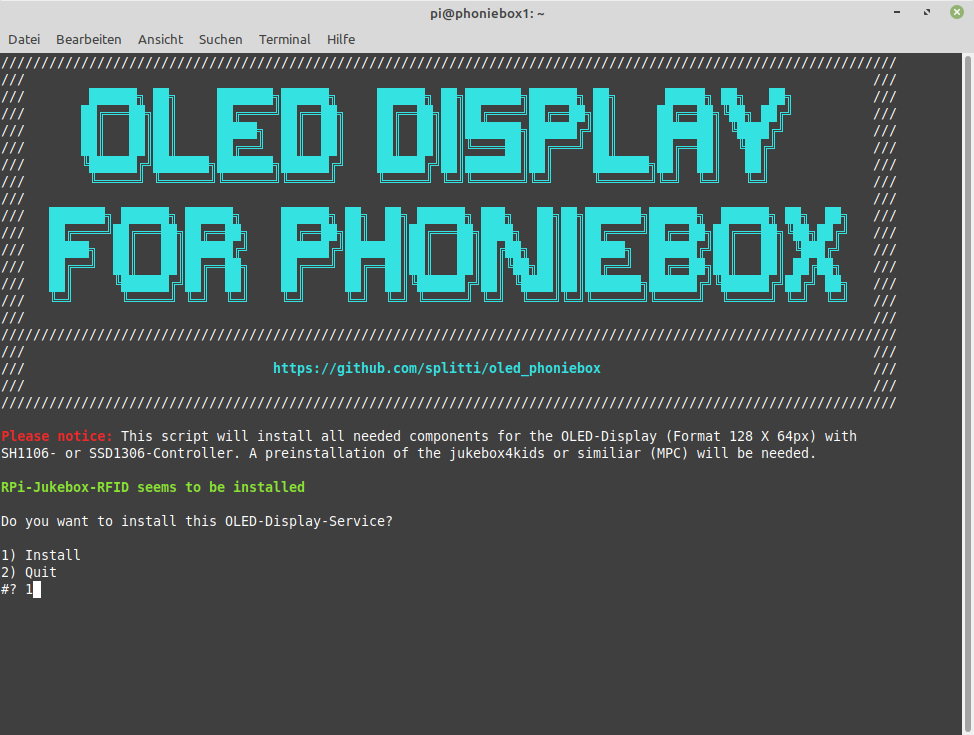
\includegraphics[width=0.47\textwidth]{/OLED/oled01.png}
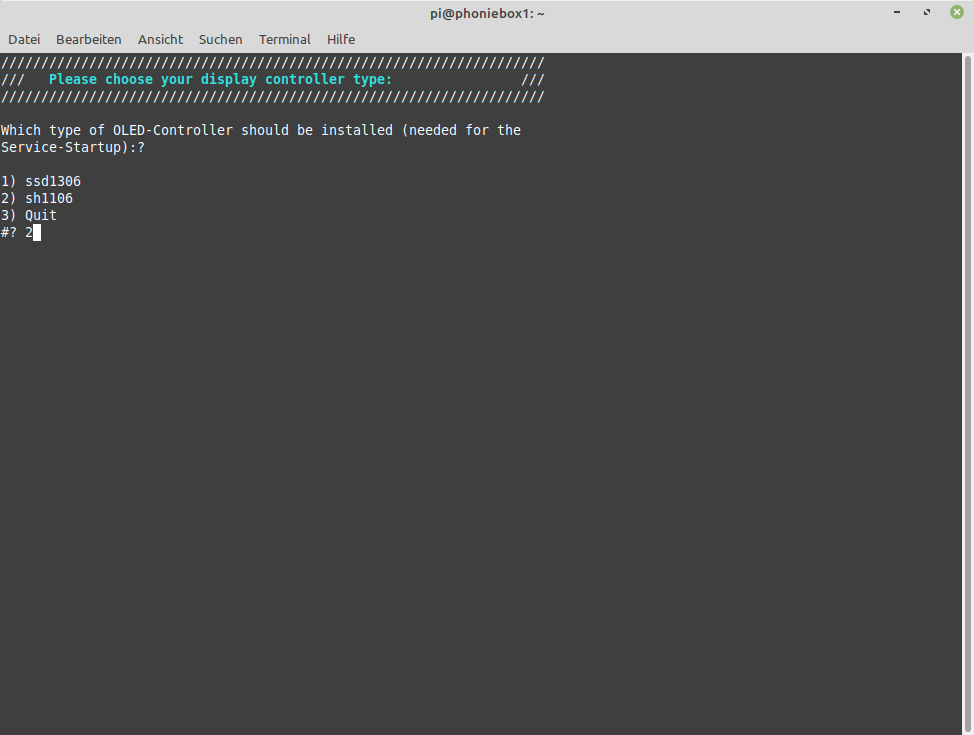
\includegraphics[width=0.47\textwidth]{/OLED/oled02.png}
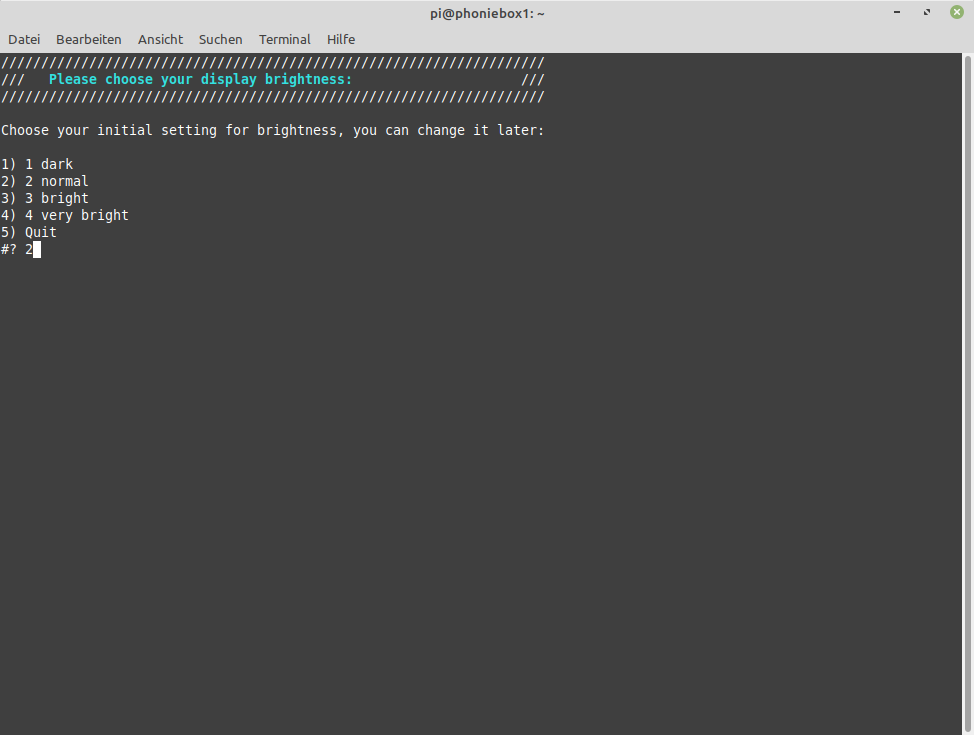
\includegraphics[width=0.47\textwidth]{/OLED/oled03.png}
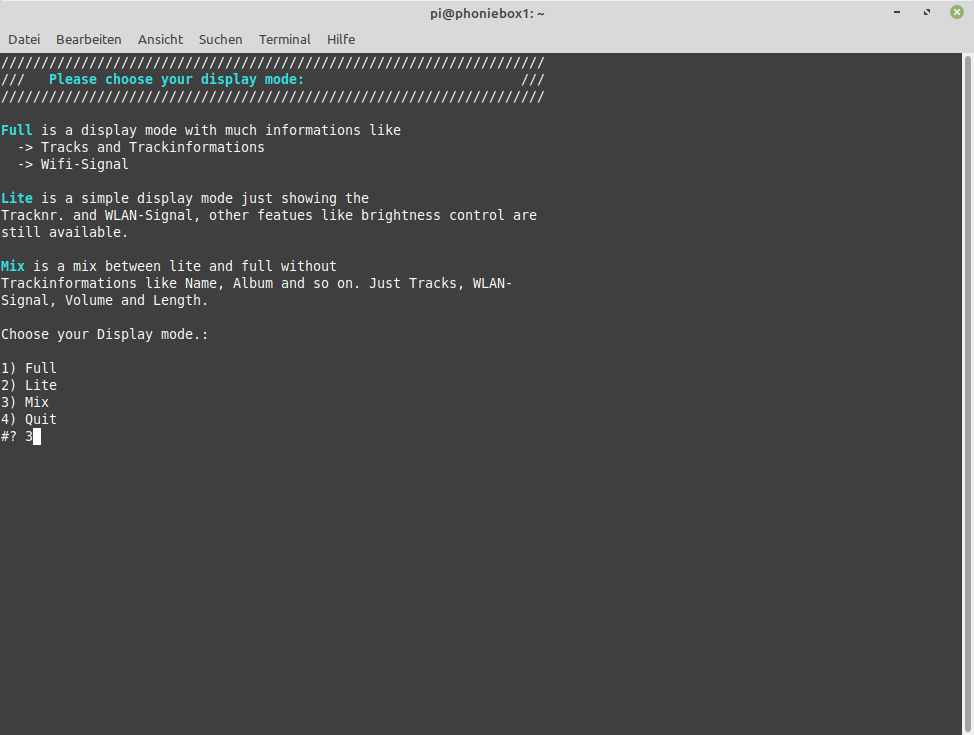
\includegraphics[width=0.47\textwidth]{/OLED/oled04.png}
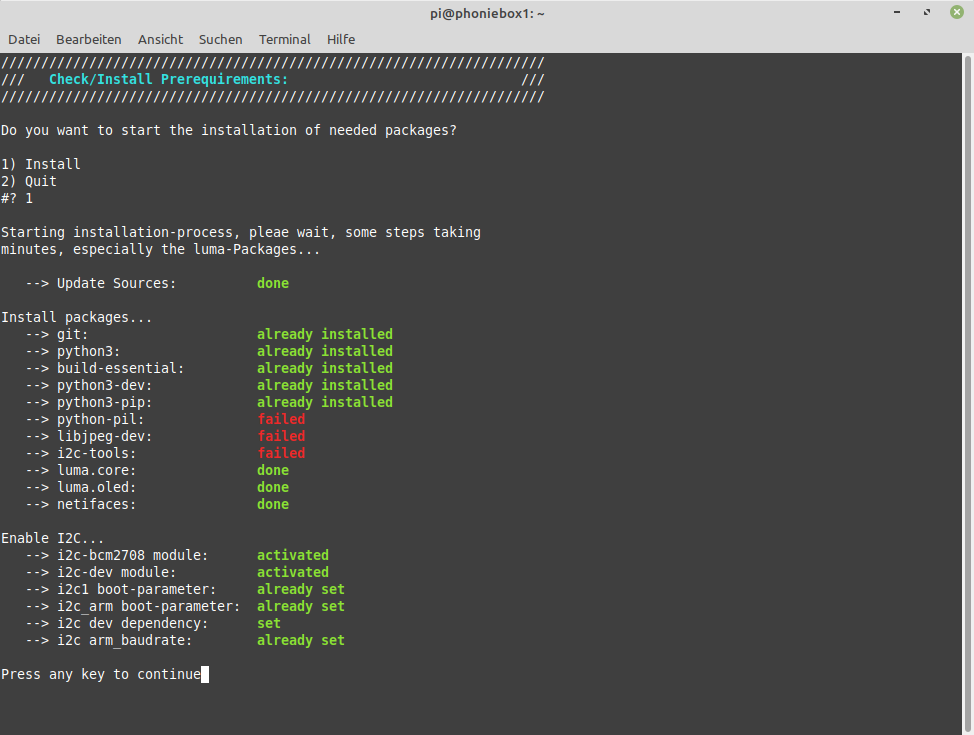
\includegraphics[width=0.47\textwidth]{/OLED/oled05.png}
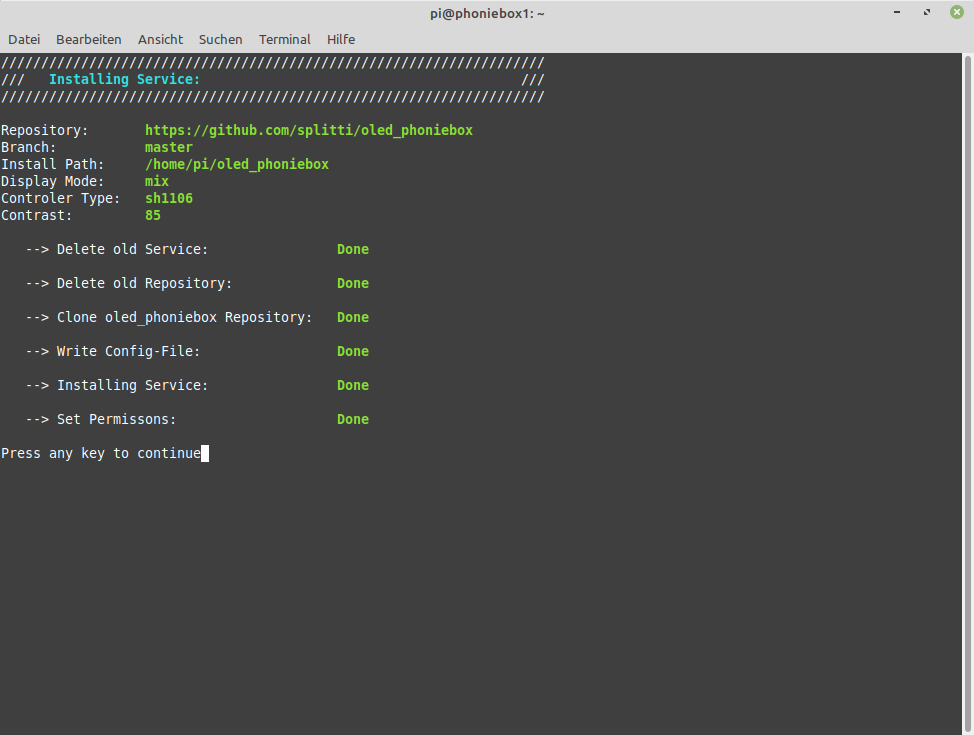
\includegraphics[width=0.47\textwidth]{/OLED/oled06.png}
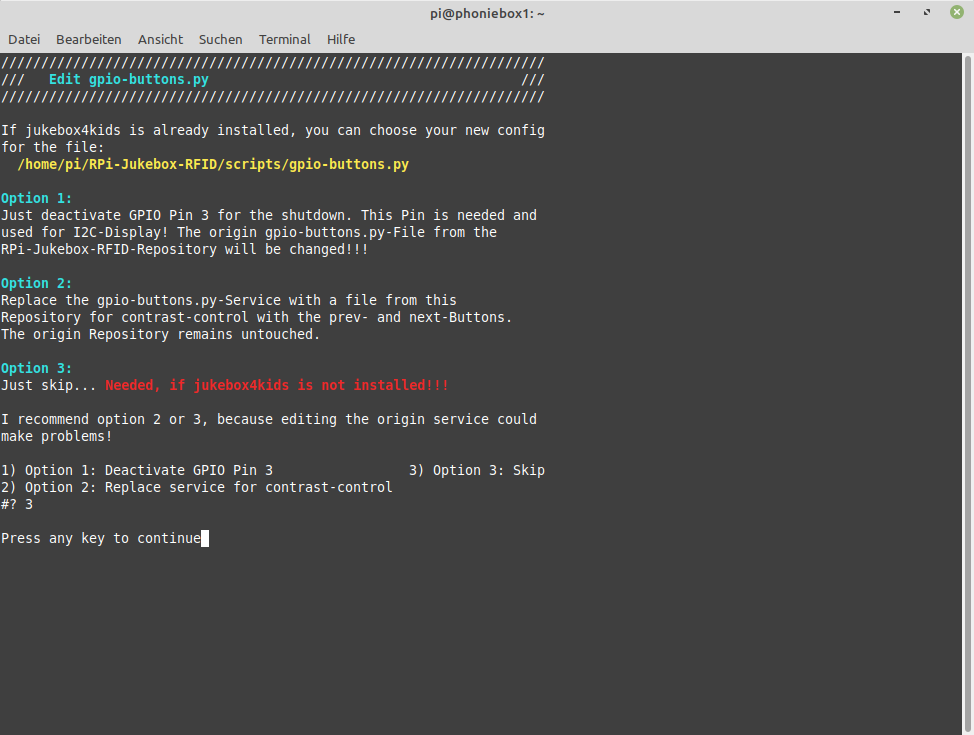
\includegraphics[width=0.47\textwidth]{/OLED/oled07.png}
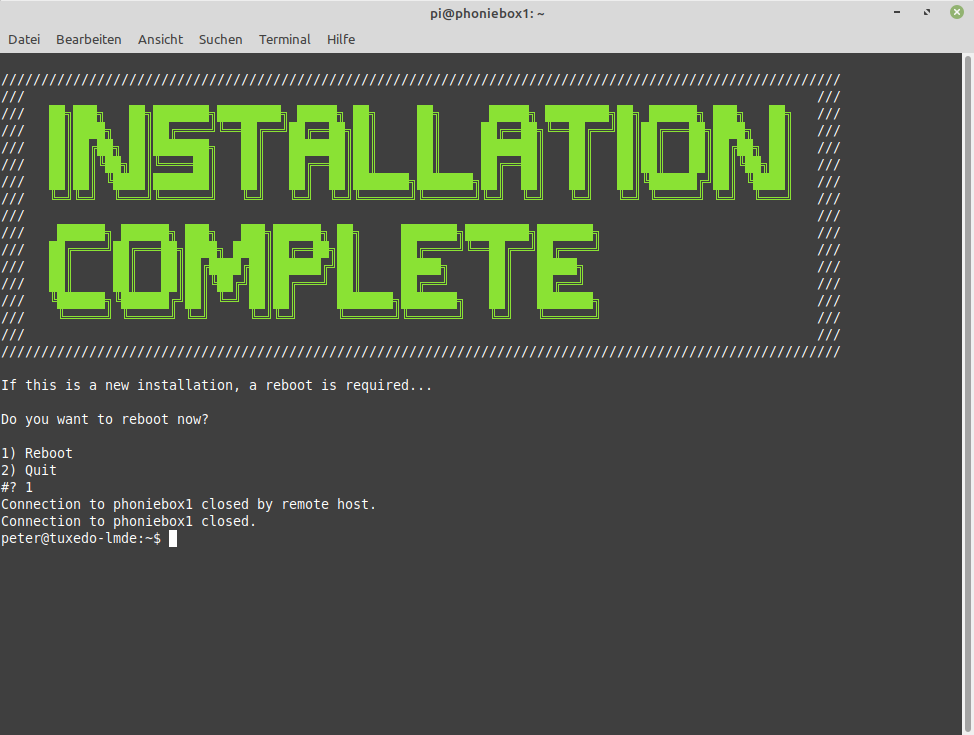
\includegraphics[width=0.47\textwidth]{/OLED/oled08.png}
\caption{splitti79s one line installer}
\end{figure}







%\section{Installation der \Bezeichnung-Software}
%bla bla
%
%
%
%
%
%\section{Software / Installation}
%ReadMe einbinden...
%
%\subsection{offen}
%Reduzierung der Bootzeit\\
%automatisch aus nach 15 min.
%
